
\chapter{Momentum balance} \label{ssn_momentum_balance}

\index{Balance equations!Momentum}
\index{Stokes equations!Slip-friction}
\index{Hydrostatic stress}
Momentum-balance equation (\ref{cons_momentum}) and mass-balance equation (\ref{cons_mass}), collectively referred to as the Stokes equations (see \S \ref{ssn_intro_stokes_2d}, \S \ref{ssn_intro_stokes_2d_slip}, \S \ref{ssn_intro_stokes_3d}, \S \ref{ssn_intro_stokes_2d_slip_stab}, and the introductory chapter of \citet{elman_2005}), are completed with boundary conditions encompassing the entire outer surface $\Gamma = \Gamma_A \cup \Gamma_W \cup \Gamma_G$, with atmospheric boundary $\Gamma_A$, boundary in contact with ocean $\Gamma_W$, basal boundary in contact with bedrock $\Gamma_G$, and complete basal boundary including floating ice $\Gamma_B$ (see Figure \ref{ice_profile_domain}).

Momentum balance (\ref{cons_momentum}) boundary conditions are naturally applied as perpendicularly-applied \emph{normal stresses},
\begin{align}
  \label{atmosphere_normal_stress}
  \big( \ranktwo{\sigma} \cdot \normal \big)_{\perp} &= - p_a \normal &&\text{ on } \Gamma_A &&\leftarrow \text{ atmosphere pres.} \\
  \label{water_normal_stress}
  \big( \ranktwo{\sigma} \cdot \normal \big)_{\perp} &= - p_w \normal &&\text{ on } \Gamma_W &&\leftarrow \text{ ocean pres.} \\
  \label{bedrock_normal_stress}
  \big( \ranktwo{\sigma} \cdot \normal \big)_{\perp} &= - p_b \normal &&\text{ on } \Gamma_B &&\leftarrow \text{ lithosphere pres.},
\end{align}
and also tangentially-applied \emph{shear stresses},
\begin{align}
  \label{atmosphere_shear_stress}
  \big( \ranktwo{\sigma} \cdot \normal \big)_{\Vert} &= - \beta_a \rankone{u}_a &&\text{ on } \Gamma_A &&\leftarrow \text{ wind shear} \\
  \label{water_shear_stress}
  \big( \ranktwo{\sigma} \cdot \normal \big)_{\Vert} &= - \beta_w \rankone{u}_w &&\text{ on } \Gamma_W &&\leftarrow \text{ ocean shear} \\
  \label{bedrock_shear_stress}
  \big( \ranktwo{\sigma} \cdot \normal \big)_{\Vert} &= - \beta_b \rankone{u}   &&\text{ on } \Gamma_G &&\leftarrow \text{ basal shear}.
\end{align}
%with outward-pointing normal vector to the boundary $\normal = [n_x\ n_y\ n_z]^\intercal$, and hydrostatic pressure
%\begin{align}
%  \label{water_pressure}
%  f_w = \rho_{sw} g (D - z), \hspace{5mm} z < D,
%\end{align}
%with seawater density $\rho_{sw}$ and ocean height $D$.

Note that the stress boundaries are applied in the direction of the outward normal, with normal components denoted $(\rankone{v})_{\perp} = \left( \rankone{v} \cdot \normal \right) \normal$ and tangential components denoted $(\rankone{v})_{\Vert} = \rankone{v} - \left( \rankone{v} \cdot \normal \right) \normal$.
In particular, tangential traction condition (\ref{basal_drag}) has been stated in proportion to the basal velocity $\rankone{u} |_{\Gamma_G}$ and basal-traction coefficient $\beta \geq 0$, while ocean-stress boundary (\ref{water_stress}) is applied normal to the surface.
The water will also apply a non-zero shearing force to the ice sheet in areas where $\beta > 0$ on $\Gamma_W$.
Finally, notice that traction boundary (\ref{basal_drag}) and impenetrability boundary (\ref{impenetrability}) are identical to slip-friction boundary conditions (\ref{intro_stokes_gN_N_S_D_fric}) and (\ref{intro_stokes_gD_N_S_D_slip}) explored previously in \S \ref{ssn_intro_stokes_2d_slip} and \S \ref{ssn_intro_stokes_2d_slip_stab}.

Throughout the following sections, Python source code associated with these fundamental equations will be provided.  For example, viscosity (\ref{viscosity}) is created using FEniCS in Code Listing \ref{viscosity_code}. 

\begin{python}[label=viscosity_code, caption={FEniCS code used to generate viscosity $\eta$ as defined in the \texttt{Momentum} class, from which all of the momentum models of this chapter inherit.}]
def viscosity(self, U):
  """
  calculates the viscosity eta.  Uses velocity vector <U> with
  components u,v,w.  If <linear> == True, form viscosity from model.U3.
  """
  s  = "::: forming viscosity :::"
  print_text(s, self.color())
  model    = self.model
  n        = model.n
  A_f      = model.A_f
  eps_reg  = model.eps_reg
  epsdot   = self.effective_strain_rate(U)
  eta      = 0.5 * A_f**(-1/n) * (epsdot + eps_reg)**((1-n)/(2*n))
  return eta
\end{python}
%===============================================================================

\section{Full-Stokes equations} \label{ssn_full_stokes}

The expanded Stokes equations are identical to (\ref{3d_stokes_expanded}), and comprise a system of four equations and four unknowns $u$, $v$, $w$, and $p$.  The complexity of solving this system and associated boundary conditions (\ref{surface_stress} -- \ref{impenetrability}) has already been explored in \S \ref{ssn_intro_stokes_2d_slip} and \S \ref{ssn_intro_stokes_2d_slip_stab}; namely, the satisfaction or circumvention of inf-sup condition (\ref{inf_sup_condition}) and the correct imposition of Dirichlet condition (\ref{impenetrability}).  An elegant method satisfying these requirements is presented in the next section.

\subsection{Variational principle} \label{ssn_full_stokes_var_prin}

\index{Variational principle!Full-Stokes}
To solve system (\ref{cons_momentum}, \ref{cons_mass}, \ref{surface_stress} -- \ref{impenetrability}),  the method described in \citet{dukowicz_2010} is used.  This method makes use of a variational principle that uniquely determines velocity $\rankone{u}$ and pressure $p$ by finding the extremum of the \emph{action integral}

\begin{align}
  \label{action}
  \pazocal{A} \left(\rankone{u}, p\right) = &+ \int_{\Omega} \left( V\left( \dot{\varepsilon}_e^2 \right) - \rho \rankone{g} \cdot \rankone{u} - p \nabla \cdot \rankone{u} \right) \d{\Omega} \notag \\
  &+ \int_{\Gamma_B} \left( \Lambda \rankone{u} \cdot \normal + \frac{1}{2} \beta \rankone{u} \cdot \rankone{u} \right) \d{\Gamma_B} \notag \\
  &+ \int_{\Gamma_W} f_w \normal \cdot \rankone{u} \d{\Gamma_W},
\end{align}
with viscous-dissipation term
\begin{align}
  \label{viscous_dissipation}
  V\left( \dot{\varepsilon}_e^2 \right) &= 2 \int_0^{\dot{\varepsilon}_e^2} \eta(s) \d{s} \notag \\
  &= A^{-\nicefrac{1}{n}} \int_0^{\dot{\varepsilon}_e^2} s^{\frac{1-n}{2n}} \d{s} \notag \\
  &= \frac{2n}{n+1} A^{-\nicefrac{1}{n}} \left( \dot{\varepsilon}_e^2 \right)^{\frac{n+1}{2n}} \notag \\
  &= \frac{2n}{n+1} \left( A^{-\nicefrac{1}{n}} \left( \dot{\varepsilon}_e^2 \right)^{\frac{1-n}{2n}} \right) \dot{\varepsilon}_e^2 \notag \\
  &= \frac{4n}{n+1} \eta\left(\theta, \rankone{u} \right) \dot{\varepsilon}_e^2,
\end{align}
where shear viscosity $\eta$ is given by (\ref{viscosity}).  Lagrange multiplier $\Lambda$ enforces basal-surface impenetrability condition (\ref{impenetrability}), while pressure $p$ -- defined as the mean compressive stress $p = -\sigma_{kk} / 3$ -- also takes on the role of a Lagrange multiplier to enforce incompressibility condition (\ref{cons_mass}).

This extremum is defined as the solution to 
\begin{align}
  \label{extremum_intermediate}
  \frac{\delta \pazocal{A}}{\delta \rankone{u}} = 0, \hspace{5mm} \frac{\delta \pazocal{A}}{\delta p} = 0, \hspace{5mm} \frac{\delta \pazocal{A}}{\delta \Lambda} = 0,
\end{align}
and has been shown to be equivalent to the Stokes system (\ref{cons_momentum}, \ref{cons_mass}) by \citet{dukowicz_2010} and boundary conditions (\ref{surface_stress} -- \ref{impenetrability}) by \citet{dukowicz_2011}.
It was also explained by \citet{dukowicz_2011} how the basal stress arising from Euler-Lagrange equations (\ref{extremum_intermediate}) is constrained to obey
\begin{align}
  \label{dukowicz_basal_stress}
  \ranktwo{\sigma} \cdot \normal \big|_{\Gamma_B} &= - \beta \rankone{u} - \Lambda \normal.
\end{align}
The magnitude of stress normal to the bed is determined by taking the dot product of (\ref{dukowicz_basal_stress}) with $\normal$, making use of bed-impenetrability condition (\ref{impenetrability}), and the definition of a unit vector, resulting in
\begin{align}
  \label{dukowicz_lambda}
  \Lambda &= - \normal \cdot \ranktwo{\sigma} \cdot \normal.
\end{align}
Therefore, $\Lambda$ is equivalent to the magnitude of stress presented by the ice on the supporting bedrock.  Relation (\ref{dukowicz_lambda}) may be used to eliminate Lagrange multiplier $\Lambda$ in (\ref{action}); hence extremum conditions (\ref{extremum_intermediate}) are reduced to
\begin{align}
  \label{extremum}
  \frac{\delta \pazocal{A}}{\delta \rankone{u}} = 0, \hspace{10mm} \frac{\delta \pazocal{A}}{\delta p} = 0.
\end{align}
Additionally, by assuming that the magnitude of the normal component of deviatoric-stress tensor (\ref{stress_tensor}), $\normal \cdot \tau \cdot \normal$, is much less than pressure $p$ along the entire basal surface $\Gamma_B$, (\ref{dukowicz_lambda}) simplifies to $\Lambda \approx p$.  This approximation has in our experience lead to improved convergence characteristics of the discrete system when the topography includes steep basal gradients.  Additionally, using both (\ref{dukowicz_basal_stress}) and (\ref{dukowicz_lambda}), observe that the tangential component of stress is
\begin{align}
  \left( \ranktwo{\sigma} \cdot \normal \right)_{\Vert} &= \ranktwo{\sigma} \cdot \normal - \left( \normal \cdot \ranktwo{\sigma} \cdot \normal\right) \normal \notag \\
  &= - \beta \rankone{u} - \Lambda \normal - \left( -\Lambda \right) \normal \notag \\
  &= - \beta \rankone{u},
\end{align}
and is thus consistent with traction-boundary-condition (\ref{basal_drag}).

The source code of \CSLVR uses an implementation similar to Code Listing \ref{cslvr_full_stokes}.

\begin{python}[label=cslvr_full_stokes, caption={\CSLVR source code contained in the \texttt{MomentumDukowiczStokes} class.}]
# define variational problem :
U                    = Function(model.Q4, name = 'G')
dU                   = TrialFunction(model.Q4)
Phi                  = TestFunction(model.Q4)
phi, psi, xi,  kappa = Phi
du,  dv,  dw,  dP    = dU
u,   v,   w,   p     = U

# create velocity vector :
U3      = as_vector([u,v,w])

# viscous dissipation :
epsdot  = self.effective_strain_rate(U3)
if linear:
  s   = "    - using linear form of momentum using model.U3 in epsdot -"
  Uc  = model.U3.copy(True)
  eta = self.viscosity(Uc)
  Vd  = 2 * eta * epsdot
else:
  s   = "    - using nonlinear form of momentum -"
  eta = self.viscosity(U3)
  Vd  = (2*n)/(n+1) * A_f**(-1/n) * (epsdot + eps_reg)**((n+1)/(2*n))
print_text(s, self.color())

# potential energy :
Pe     = - rhoi * g * w

# dissipation by sliding :
Ut     = U3 - dot(U3,N)*N
Sl     = - 0.5 * beta * dot(Ut, Ut)

# incompressibility constraint :
Pc     = p * div(U3)

# impenetrability constraint :
sig    = self.stress_tensor(U3, p, eta)
lam    = - dot(N, dot(sig, N))
Nc     = - lam * (dot(U3, N) - Fb)

# pressure boundary :
Pb_w   = - rhosw*g*D * dot(U3, N)

# action integral :
A      = + (Vd - Pe - Pc)*dx - Nc*dBed \
         - Sl*dBed_g - Pb_w*dBed_f - Pb_w*dLat_t

# the first variation of the action integral in the direction of a 
# test function; the extremum :
self.mom_F = derivative(A, U, Phi)

# the first variation of the extremum in the direction 
# a trial function; the Jacobian :
self.mom_Jac = derivative(self.mom_F, U, dU)

def stress_tensor(self, U, p, eta):
  """
  return the Cauchy stress tensor.
  """
  s   = "::: forming the Cauchy stress tensor :::"
  print_text(s, self.color())

  I     = Identity(3)
  tau   = self.deviatoric_stress_tensor(U, eta)

  sigma = tau - p*I
  return sigma

def deviatoric_stress_tensor(self, U, eta):
  """
  return the deviatoric stress tensor.
  """
  s   = "::: forming the deviatoric part of the Cauchy stress tensor :::"
  print_text(s, self.color())

  epi = self.strain_rate_tensor(U)
  tau = 2 * eta * epi
  return tau

def strain_rate_tensor(self, U):
  """
  return the strain-rate tensor of <U>.
  """
  epsdot = 0.5 * (grad(U) + grad(U).T)
  return epsdot

def effective_strain_rate(self, U):
  """
  return the effective strain rate squared.
  """
  epi    = self.strain_rate_tensor(U)
  ep_xx  = epi[0,0]
  ep_yy  = epi[1,1]
  ep_zz  = epi[2,2]
  ep_xy  = epi[0,1]
  ep_xz  = epi[0,2]
  ep_yz  = epi[1,2]
  
  # Second invariant of the strain rate tensor squared
  epsdot = 0.5 * (+ ep_xx**2 + ep_yy**2 + ep_zz**2) \
                  + ep_xy**2 + ep_xz**2 + ep_yz**2
  return epsdot

def default_solve_params(self):
  """ 
  Returns a set of default solver parameters that yield good performance
  """
  nparams = {'newton_solver' :
            {
              'linear_solver'            : 'mumps',
              'relative_tolerance'       : 1e-5,
              'relaxation_parameter'     : 0.7,
              'maximum_iterations'       : 25,
              'error_on_nonconvergence'  : False,
            }}
  m_params  = {'solver'      : nparams}
  return m_params

def solve(self, annotate=False):
  """ 
  Perform the Newton solve of the full-Stokes equations 
  """
  # zero out self.velocity for good convergence for any subsequent solves,
  # e.g. model.L_curve() :
  model.assign_variable(self.get_U(), DOLFIN_EPS, cls=self)
  
  # compute solution :
  solve(self.mom_F == 0, self.U, J = self.mom_Jac, bcs = self.mom_bcs,
        annotate = annotate, solver_parameters = params['solver'])
  u, v, w, p = self.U.split()
  
\end{python}

\section{First-order approximation} \label{ssn_first_order}

\index{Stokes equations!Applied to ice, first-order}
\index{Stokes equations!Slip-friction}
Assumptions pertaining to both the state of stress and strain are appropriate over a large proportion of ice-sheets, and lead to considerable simplifications of full-Stokes equations (\ref{stokes_exp}).  These simplifications and associated variational principle are described here.

\subsection{Stress tensor simplification}

The Stokes equations with four equations and four unknowns $u$, $v$, $w$, and $p$ may be reduced to a system of three equations for the velocity components alone, as given by \citet{blatter_1995} and \citet{pattyn_2003}.  This is accomplished by first assuming that the shear stress components in the $z$-coordinate plane are negligible when compared to the $z$-coordinate normal stress, \ie $\partial_x \sigma_{zx}, \partial_y \sigma_{zy} \ll \partial_z \sigma_{zz}$.  Using this assumption, the final equation arising from the expansion of momentum-conservation relation (\ref{cons_momentum}), Equation (\ref{third_stokes_exp}), is reduced to
\begin{align}
  \label{stress_tensor_simplification}
  \parder{\sigma_{zz}}{z} &\approx \rho g,
\end{align}
which may be integrated from the surface to an arbitrary $z$-coordinate,
\begin{align*}
  \int_z^S \parder{\sigma_{zz}}{z} \d{z'} &\approx \int_z^S \rho g \d{z'} \\
  \sigma_{zz}(S) - \sigma_{zz}(z) &\approx \rho g (S - z).
\end{align*}
Using surface-stress condition (\ref{surface_stress}), $\sigma_{zz}(S) = 0$, and applying Cauchy-stress tensor definition (\ref{stress_tensor}),
\begin{align}
  \label{bp_pressure}
  p(z) &\approx \rho g(S - z) + 2\eta \parder{w}{z}(z).
\end{align}
This pressure approximation may then be used to eliminate $p$ from the remaining pressure derivative terms in momentum-balance (\ref{cons_momentum}) with
\begin{align}
  \label{bp_pressure_gradient}
  \parder{p}{i} &\approx
  \rho g\parder{S}{i} + \parder{}{i} \left[ 2\eta \parder{w}{z} \right], \hspace{5mm} i \in x,y.
\end{align}
allowing the simplification of (\ref{first_stokes_exp}) to
{\tiny
\begin{align}
  \parder{}{x} \left[2\eta \parder{u}{x} \right]  - \parder{p}{x} + \parder{}{y} \left[\eta \left( \parder{u}{y} + \parder{v}{x} \right) \right] + \parder{}{z} \left[\eta \left( \parder{u}{z} + \parder{w}{x} \right) \right] &= 0 \notag \\ 
  \parder{}{x} \left[2\eta \parder{u}{x} \right]  - \rho g\parder{S}{x} + \parder{}{x} \left[ 2\eta \parder{w}{z} \right] + \parder{}{y} \left[\eta \left( \parder{u}{y} + \parder{v}{x} \right) \right] & \notag \\
  + \parder{}{z} \left[\eta \left( \parder{u}{z} + \parder{w}{x} \right) \right] &= 0 \notag \\ 
  \label{first_stokes_exp_stress_simp}
  \parder{}{x} \left[2\eta \left( \parder{u}{x} - \parder{w}{z} \right) \right]  + \parder{}{y} \left[\eta \left( \parder{u}{y} + \parder{v}{x} \right) \right] + \parder{}{z} \left[\eta \left( \parder{u}{z} + \parder{w}{x} \right) \right] &= \rho g\parder{S}{x},
\end{align}}
and (\ref{second_stokes_exp}) to
{\tiny
\begin{align}
  \parder{}{x} \left[\eta \left( \parder{v}{x} + \parder{u}{y} \right) \right]  + \parder{}{y} \left[2\eta \parder{v}{y} \right] - \parder{p}{y} + \parder{}{z} \left[\eta \left( \parder{v}{z} + \parder{w}{y} \right) \right] &= 0 \notag \\ 
  \parder{}{x} \left[\eta \left( \parder{v}{x} + \parder{u}{y} \right) \right]  + \parder{}{y} \left[2\eta \parder{v}{y} \right] - \rho g\parder{S}{y} + \parder{}{y} \left[ 2\eta \parder{w}{z} \right] &\notag \\
  + \parder{}{z} \left[\eta \left( \parder{v}{z} + \parder{w}{y} \right) \right] &= 0 \notag \\ 
  \label{second_stokes_exp_stress_simp}
  \parder{}{x} \left[\eta \left( \parder{v}{x} + \parder{u}{y} \right) \right]  + \parder{}{y} \left[2\eta \left( \parder{v}{y} - \parder{w}{z} \right) \right] + \parder{}{z} \left[\eta \left( \parder{v}{z} + \parder{w}{y} \right) \right] &= \rho g \parder{S}{y},
\end{align}}
which combined with conservation of mass relation (\ref{fourth_stokes_exp}),
\begin{align*}
  \parder{u}{x} + \parder{v}{y} + \parder{w}{z} &= 0 && \text{in } \Omega 
\end{align*}
gives three equations and three unknowns $u$, $v$, and $w$.

\subsection{Strain tensor simplification} \label{ssn_strain_tensor_simplification}

Next, assuming the horizontal gradients of $w$ are much less than the vertical gradient of the horizontal components of velocity, \ie $\partial_x w \ll \partial_z u$ and $\partial_y w \ll \partial_z v$, and using (\ref{stress_tensor_simplification}), strain-rate tensor (\ref{strain_rate_tensor}) is decoupled from vertical velocity $w$, resulting in the strain-rate quasi-tensor
\begin{align}
  \label{bp_strain_rate_tensor}
  \tilde{\ranktwo{\dot{\epsilon}}}
  &= \begin{bmatrix}
       \parder{u}{x} & \frac{1}{2}\left( \parder{u}{y} + \parder{v}{x} \right) & \frac{1}{2} \parder{u}{z} \\
       \frac{1}{2}\left( \parder{v}{x} + \parder{u}{y} \right) & \parder{v}{y} & \frac{1}{2} \parder{v}{z} \\
     \end{bmatrix}.
\end{align}
Effective strain-rate (\ref{effective_strain_rate}) is also decoupled from $w$ using the equivalent relation to conservation of mass relation (\ref{cons_mass}), $\dot{\epsilon}_{zz} = -\left(\dot{\epsilon}_{xx} + \dot{\epsilon}_{yy} \right)$,
\begin{align}
  \label{bp_effective_strain_rate}
  \dot{\varepsilon}_{\text{BP}}^2 = \tilde{\dot{\epsilon}}_{xx}^2 + \tilde{\dot{\epsilon}}_{yy}^2 + \tilde{\dot{\epsilon}}_{xx} \tilde{\dot{\epsilon}}_{yy} + \tilde{\dot{\epsilon}}_{xy}^2 + \tilde{\dot{\epsilon}}_{xz}^2 + \tilde{\dot{\epsilon}}_{yz}^2.
\end{align}
Using first-order effective strain-rate (\ref{bp_effective_strain_rate}), the associated first-order shear viscosity is
\begin{align}
  \label{bp_viscosity}
  \eta_{\text{BP}}(\theta, \rankone{u}_h) &= \frac{1}{2}A(\theta)^{-\nicefrac{1}{n}} (\dot{\varepsilon}_{\text{BP}} + \dot{\varepsilon}_0)^{\frac{1-n}{n}},
\end{align} 
where horizontal vector components are denoted $\rankone{g}_h = [g_x\ g_y]^\intercal$.

Finally, inserting pressure derivative approximation (\ref{bp_pressure_gradient}) and first-order strain-rate quasi-tensor (\ref{bp_strain_rate_tensor}) into conservation of momentum relation (\ref{cons_momentum}), simplification (\ref{first_stokes_exp_stress_simp}) becomes
{\tiny
\begin{align}
  \parder{}{x} \left[2\eta \left( \parder{u}{x} - \parder{w}{z} \right) \right]  + \parder{}{y} \left[\eta \left( \parder{u}{y} + \parder{v}{x} \right) \right] + \parder{}{z} \left[\eta \left( \parder{u}{z} + \parder{w}{x} \right) \right] &= \rho g\parder{S}{x} \notag \\
  \parder{}{x} \left[2\eta \left( \parder{u}{x} + \left( \parder{u}{x} + \parder{v}{y} \right)\right) \right]  + \parder{}{y} \left[\eta \left( \parder{u}{y} + \parder{v}{x} \right) \right] + \parder{}{z} \left[\eta \parder{u}{z} \right] &= \rho g\parder{S}{x} \notag \\
  \label{first_stokes_exp_strain_simp}
  \parder{}{x} \left[2\eta \left( 2\parder{u}{x} + \parder{v}{y} \right) \right]  + \parder{}{y} \left[\eta \left( \parder{u}{y} + \parder{v}{x} \right) \right] + \parder{}{z} \left[\eta \parder{u}{z} \right] &= \rho g\parder{S}{x}
\end{align}}
and simplification (\ref{second_stokes_exp_stress_simp}) becomes 
{\tiny
\begin{align}
  \parder{}{x} \left[\eta \left( \parder{v}{x} + \parder{u}{y} \right) \right]  + \parder{}{y} \left[2\eta \left( \parder{v}{y} - \parder{w}{z} \right) \right] + \parder{}{z} \left[\eta \left( \parder{v}{z} + \parder{w}{y} \right) \right] &= \rho g \parder{S}{y} \notag \\
  \parder{}{x} \left[\eta \left( \parder{v}{x} + \parder{u}{y} \right) \right]  + \parder{}{y} \left[2\eta \left( \parder{v}{y} + \left(\parder{u}{x} + \parder{v}{y} \right)\right) \right] + \parder{}{z} \left[\eta \parder{v}{z} \right] &= \rho g \parder{S}{y} \notag \\
  \label{second_stokes_exp_strain_simp}
  \parder{}{x} \left[\eta \left( \parder{v}{x} + \parder{u}{y} \right) \right]  + \parder{}{y} \left[2\eta \left( 2\parder{v}{y} + \parder{u}{x} \right) \right] + \parder{}{z} \left[\eta \parder{v}{z} \right] &= \rho g \parder{S}{y},
\end{align}}
two equations and two unknowns $u$ and $v$.  The first-order momentum balance is therefore
\begin{align}
  \label{bp_cons_momentum}
  \nabla \cdot \ranktwo{\sigma}_{\text{BP}} &= \rho g (\nabla S)_h &&\text{ in } \Omega,
\end{align}
with Blatter-Pattyn stress quasi-tensor
\begin{align}
  \label{bp_stress_tensor}
  \ranktwo{\sigma}_{\text{BP}} &=
  2 \eta_{\text{BP}} 
  \begin{bmatrix}
       \left( 2\parder{u}{x} + \parder{v}{y} \right) & \frac{1}{2}\left( \parder{u}{y} + \parder{v}{x} \right) & \frac{1}{2} \parder{u}{z} \\
       \frac{1}{2}\left( \parder{v}{x} + \parder{u}{y} \right) & \left( 2\parder{v}{y} + \parder{u}{x} \right) & \frac{1}{2} \parder{v}{z}
     \end{bmatrix}.
\end{align}

\subsection{First-order vertical velocity and boundary conditions}

Because vertical velocity $w$ has been eliminated from conservation of momentum (\ref{cons_momentum}) through the creation of first-order momentum balance (\ref{bp_cons_momentum}), this component of velocity may be computed directly by integrating conservation of mass (\ref{cons_mass}) vertically, resulting in
\begin{align}
  \label{bp_vertical_velocity}
  w(z) &= w(B) - \int_B^z \left( \parder{u}{x} + \parder{v}{y} \right) \d{z'},
\end{align}
where the basal vertical velocity is determined directly from impenetrability condition \index{Impenetrability} (\ref{impenetrability}),
\begin{align}
  \label{bp_bed_vertical_velocity}
  w(B) &= - \frac{u(B) n_x + v(B) n_y}{n_z}. 
\end{align}
Finally, because both incompressibility (\ref{cons_mass}) and impenetrability (\ref{impenetrability}) are enforced by vertical velocity relation (\ref{bp_vertical_velocity}, \ref{bp_bed_vertical_velocity}), the remaining first-order boundary conditions are
\begin{align}
  \label{bp_exterior_stress}
  \ranktwo{\sigma}_{\text{BP}} \cdot \normal &= f_e \normal_h &&\text{ on } \Gamma_E &&\leftarrow \text{ exterior stress} \\
  \label{bp_basal_drag}
  \ranktwo{\sigma}_{\text{BP}} \cdot \normal &= -\beta \rankone{u}_h &&\text{ on } \Gamma_G &&\leftarrow \text{ basal traction},
\end{align}
where exterior stress condition (\ref{bp_exterior_stress}) is defined over exterior boundary $\Gamma_E = \Gamma_A \cup \Gamma_W$ with pressure $f_e$ derived by combining pressure approximation (\ref{bp_pressure}) and first-order stress tensor (\ref{bp_stress_tensor}) with water pressure (\ref{water_pressure}), \index{Cryostatic stress}
\begin{align}
  \label{exterior_pressure}
  f_e = f_c - f_w, \hspace{10mm} f_c = \rho g (S - z).
\end{align}
Note that boundaries located on the upper surface of the ice correspond with $f_e = 0$ and are thus stress-free, while cliff faces have $z \neq S$ and hence $f_c \neq 0$ (see Figure \ref{ice_profile_domain}).

\subsection{First-order variational principle} \label{ssn_first_order_var_prin}

\index{Variational principle!First-order}
Also compiled by \citet{dukowicz_2011} is a first-order variational principle for first-order momentum balance (\ref{bp_cons_momentum}) and associated boundary conditions (\ref{bp_exterior_stress}, \ref{bp_basal_drag}),
\begin{align}
  \label{bp_extremum}
  \frac{\delta \pazocal{A}_{\text{BP}}}{\delta \rankone{u}_h} = 0, \hspace{10mm} \frac{\delta \pazocal{A}_{\text{BP}}}{\delta \Lambda_{\text{BP}}} = 0.
\end{align}
where
\begin{align}
  \label{bp_action}
  \pazocal{A}_{\text{BP}} \left(\rankone{u}_h \right) = &+ \int_{\Omega} \left( V\left( \dot{\varepsilon}_{\text{BP}}^2 \right) + \rho g \rankone{u}_h \cdot (\nabla S)_h \right) \d{\Omega} \notag \\
  &+ \int_{\Gamma_B} \left( \Lambda_{\text{BP}} \rankone{u}_h \cdot \normal_h + \frac{1}{2} \beta \rankone{u}_h \cdot \rankone{u}_h \right) \d{\Gamma_B} \notag \\
  &+ \int_{\Gamma_E} f_e \normal_h \cdot \rankone{u}_h \d{\Gamma_E}, \\
  \label{bp_viscous_dissipation}
  V\left( \dot{\varepsilon}_{\text{BP}}^2 \right) = & 2 \int_0^{\dot{\varepsilon}_{\text{BP}}^2} \eta_{\text{BP}}(s) \d{s} = \frac{4n}{n+1} \eta_{\text{BP}}\left(\theta, \rankone{u}_h \right) \dot{\varepsilon}_{\text{BP}}^2,
\end{align}
and $\Lambda_{\text{BP}}$ defined similarly to (\ref{dukowicz_lambda}),
\begin{align}
  \label{bp_dukowicz_lambda}
  \Lambda_{\text{BP}} = - \normal \cdot \ranktwo{\sigma}_{\text{BP}} \cdot \normal \approx 0.
\end{align}

The source code of \CSLVR includes an implementation similar to Code Listing \ref{cslvr_first_order}.

\begin{python}[label=cslvr_first_order, caption={\CSLVR source code contained in the \texttt{MomentumDukowiczBP} class.}]
# define variational problem :
U        = Function(model.Q2, name = 'G')
dU       = TrialFunction(model.Q2)
Phi      = TestFunction(model.Q2)
phi, psi = Phi
du,  dv  = dU
u,   v   = U

# vertical velocity :
dw     = TrialFunction(model.Q)
chi    = TestFunction(model.Q)
w      = Function(model.Q, name='w_f')

# viscous dissipation :
U3     = as_vector([u,v,0])
epsdot = self.effective_strain_rate(U3)
if linear:
  s  = "    - using linear form of momentum using model.U3 in epsdot -"
  U3_c = model.U3.copy(True)
  eta  = self.viscosity(U3_c)
  Vd   = 2 * eta * epsdot
else:
  s  = "    - using nonlinear form of momentum -"
  eta  = self.viscosity(U3)
  Vd   = (2*n)/(n+1) * A_f**(-1/n) * (epsdot + eps_reg)**((n+1)/(2*n))
print_text(s, self.color())
  
# potential energy :
Pe     = - rhoi * g * (u*S.dx(0) + v*S.dx(1))

# dissipation by sliding :
Sl     = - 0.5 * beta * (u**2 + v**2)

# pressure boundary :
Pb     = (rhoi*g*(S - z) - rhosw*g*D) * (u*N[0] + v*N[1])

# action integral :
A      = + (Vd_gnd - Pe)*dx - Sl*dBed_g - Pb*dBed_f - Pb*dLat_t

# the first variation of the action integral in the direction of a 
# test function; the extremum :
self.mom_F = derivative(A, U, Phi)

# the first variation of the extremum in the direction 
# a tril function; the Jacobian :
self.mom_Jac = derivative(self.mom_F, U, dU)

self.w_F = + (u.dx(0) + v.dx(1) + dw.dx(2))*chi*dx \
           + (u*N[0] + v*N[1] + dw*N[2] - Fb)*chi*dBed
 
def strain_rate_tensor(self, U):
  """
  return the Dukowicz 'Blatter-Pattyn' simplified strain-rate tensor of <U>.
  """
  u,v,w  = U
  epi    = 0.5 * (grad(U) + grad(U).T)
  epi02  = 0.5*u.dx(2)
  epi12  = 0.5*v.dx(2)
  epi22  = -u.dx(0) - v.dx(1)  # incompressibility
  epsdot = as_matrix([[epi[0,0],  epi[0,1],  epi02],
                      [epi[1,0],  epi[1,1],  epi12],
                      [epi02,     epi12,     epi22]])
  return epsdot
  
def effective_strain_rate(self, U):
  """
  return the Dukowicz BP effective strain rate squared.
  """
  epi    = self.strain_rate_tensor(U)
  ep_xx  = epi[0,0]
  ep_yy  = epi[1,1]
  ep_zz  = epi[2,2]
  ep_xy  = epi[0,1]
  ep_xz  = epi[0,2]
  ep_yz  = epi[1,2]
  
  # Second invariant of the strain rate tensor squared
  epsdot = + ep_xx**2 + ep_yy**2 + ep_xx*ep_yy \
           + ep_xy**2 + ep_xz**2 + ep_yz**2
  return epsdot

def default_solve_params(self):
  """ 
  Returns a set of default solver parameters that yield good performance
  """
  nparams = {'newton_solver' :
            {
              'linear_solver'            : 'cg',
              'preconditioner'           : 'hypre_amg',
              'relative_tolerance'       : 1e-5,
              'relaxation_parameter'     : 0.7,
              'maximum_iterations'       : 25,
              'error_on_nonconvergence'  : False,
              'krylov_solver'            :
              {
                'monitor_convergence'   : False,
              }
            }}
  return m_params

def solve_pressure(self, annotate=False):
  """
  Solve for the Dukowicz BP pressure to model.p.
  """
  p   = project(rhoi*g*(S - z) + 2*eta*w.dx(2),
                annotate=annotate)


def solve_vert_velocity(self, annotate=False):
  """

  Perform the Newton solve of the first-order equations 
  """
  aw       = assemble(lhs(self.w_F))
  Lw       = assemble(rhs(self.w_F))
  w_solver = LUSolver(self.solve_params['vert_solve_method'])
  w_solver.solve(aw, self.w.vector(), Lw, annotate=annotate)
  
def solve(self, annotate=False):
  """ 
  Perform the Newton solve of the first-order equations 
  """
  # zero out self.velocity for good convergence for any subsequent solves,
  # e.g. model.L_curve() :
  model.assign_variable(self.get_U(), DOLFIN_EPS, cls=self)
  
  # compute solution :
  solve(self.mom_F == 0, self.U, J = self.mom_Jac,
        annotate = annotate, solver_parameters = params['solver'])
  u, v = self.U.split()
\end{python}

\section{Plane-strain approximation} \label{ssn_plane_strain}

\index{Stokes equations!Applied to ice, plane-strain}
\index{Stokes equations!Slip-friction}
Many observations of the ice lie along $x,y$-coordinate transects.  In order to explain these observations, the \emph{plane-strain} momentum balance model \citep{hill_1950} has been formulated for ice, and is based on the assumption that longitudinal stress and lateral shear are present only in the direction of velocity $\rankone{u}$.  Using this model with flow specified in the $x$-direction, all $y$-component terms of stress tensor (\ref{stress_tensor}) and strain-rate tensor (\ref{strain_rate_tensor}) are eliminated, producing the two-dimensional model tensors \index{Tensor!Plane-strain stress} \index{Tensor!Plane-strain stain rate}
\begin{align}
  \label{ps_tensors}
  \ranktwo{\sigma}_{\text{PS}} = \begin{bmatrix}
             \sigma_{xx} & \sigma_{xz} \\
             \sigma_{zx} & \sigma_{zz}
           \end{bmatrix}, \hspace{5mm} \text{and} \hspace{5mm}
  \tilde{\ranktwo{\dot{\epsilon}}} = \begin{bmatrix}
                             \dot{\epsilon}_{xx} & \dot{\epsilon}_{xz} \\
                             \dot{\epsilon}_{zx} & \dot{\epsilon}_{zz}
                           \end{bmatrix}.
\end{align}
Effective strain-rate (\ref{effective_strain_rate}) is therefore reduced to
\begin{align}
  \label{ps_effective_strain_rate}
  \dot{\varepsilon}_{\text{PS}}^2 = &\frac{1}{2} \Bigg[ \tilde{\dot{\epsilon}}_{xx}^2 + \tilde{\dot{\epsilon}}_{zz}^2 + 2\tilde{\dot{\epsilon}}_{xz}^2 \Bigg],
\end{align}
which is used within the plane-strain viscosity
\begin{align}
  \label{ps_viscosity}
  \eta_{\text{PS}}(\theta, \rankone{u}_p) &= \frac{1}{2}A(\theta)^{-\nicefrac{1}{n}} (\dot{\varepsilon}_{\text{PS}} + \dot{\varepsilon}_0)^{\frac{1-n}{n}},
\end{align} 
with $xz$-plane velocity $\rankone{u}_p = [u\ w]\T$.  The plane-strain Stokes system analogous to full-Stokes system (\ref{cons_momentum}, \ref{cons_mass}, \ref{surface_stress} -- \ref{impenetrability}) with stress tensor $\ranktwo{\sigma}_{\text{PS}} = 2\eta_{\text{PS}} \tilde{\ranktwo{\dot{\epsilon}}} - p \ranktwo{I}$ consists of
{\small
\begin{align}
  \label{ps_cons_momentum}
  -\nabla \cdot \ranktwo{\sigma}_{\text{PS}} &= \rho\rankone{g}_p &&\text{ in } \Omega &&\leftarrow \text{ momentum} \\
  \label{ps_cons_mass}
  \nabla \cdot \rankone{u}_p &= 0 &&\text{ in } \Omega &&\leftarrow \text{ mass}  \\
  \label{ps_surface_stress}
  \ranktwo{\sigma}_{\text{PS}} \cdot \normal_p &= \rankone{0}_p &&\text{ on } \Gamma_A &&\leftarrow \text{ stress-free surf.} \\
  \label{ps_water_stress}
  \ranktwo{\sigma}_{\text{PS}} \cdot \normal_p &= -f_w \normal_p &&\text{ on } \Gamma_W &&\leftarrow \text{ water pressure} \\
  \label{ps_basal_drag}
  \big( \ranktwo{\sigma}_{\text{PS}} \cdot \normal_p \big)_{\Vert} &= -\beta \rankone{u}_p &&\text{ on } \Gamma_G &&\leftarrow \text{ basal traction } \\
  \label{ps_impenetrability}
  \rankone{u}_p \cdot \normal_p &= 0 &&\text{ on } \Gamma_B &&\leftarrow \text{ impenetrability,}
\end{align}}
with outward-pointing normal vector to the boundary $\normal_p = [n_x\ n_z]^\intercal$, gravitational acceleration vector $\rankone{g}_p = [0\ \text{-}g]\T$, water pressure $f_w$ as defined by (\ref{water_pressure}), and basal-traction coefficient $\beta \geq 0$.

\subsection{Plane-strain variational principle} \label{ssn_plane_strain_var_prin}

\index{Variational principle!Plane-strain}
Proceeding in an identical fashion as \S \ref{ssn_full_stokes_var_prin} and \S \ref{ssn_first_order_var_prin}, the associated action integral for plane-strain momentum balance (\ref{ps_cons_momentum} -- \ref{ps_impenetrability}) is
\begin{align}
  \label{ps_action}
  \pazocal{A}_{\text{PS}} \left(\rankone{u}_p, p\right) = &+ \int_{\Omega} \left( V\left( \dot{\varepsilon}_{\text{PS}}^2 \right) - \rho \rankone{g}_p \cdot \rankone{u}_p - p \nabla \cdot \rankone{u}_p \right) \d{\Omega} \notag \\
  &+ \int_{\Gamma_B} \left( \Lambda_{\text{PS}} \rankone{u}_p \cdot \normal_p + \frac{1}{2} \beta \rankone{u}_p \cdot \rankone{u}_p \right) \d{\Gamma_B} \notag \\
  &+ \int_{\Gamma_W} f_w \normal_p \cdot \rankone{u}_p \d{\Gamma_W},
\end{align}
where $\Lambda_{\text{PS}}$ is defined similarly to (\ref{dukowicz_lambda}) and (\ref{bp_dukowicz_lambda}),
\begin{align}
  \label{ps_dukowicz_lambda}
  \Lambda_{\text{PS}} = - \normal_p \cdot \ranktwo{\sigma}_{\text{PS}} \cdot \normal_p \approx p.
\end{align}
and with viscous dissipation term $V\left( \dot{\varepsilon}_{\text{PS}}^2 \right)$ defined from the same process leading to (\ref{viscous_dissipation}) and (\ref{bp_viscous_dissipation}), 
\begin{align}
  \label{ps_viscous_dissipation}
  V\left( \dot{\varepsilon}_{\text{PS}}^2 \right) &= 2 \int_0^{\dot{\varepsilon}_{\text{PS}}^2} \eta_{\text{PS}}(s) \d{s} = \frac{4n}{n+1} \eta_{\text{PS}}\left(\theta, \rankone{u}_p \right) \dot{\varepsilon}_{\text{PS}}^2.
\end{align}
Finally, the extremum of action integral (\ref{ps_action}) is given by the solution $(\rankone{u}_p, p)$ of
\begin{align}
  \label{ps_extremum}
  \frac{\delta \pazocal{A}_{\text{PS}}}{\delta \rankone{u}_p} = 0, \hspace{10mm} \frac{\delta \pazocal{A}_{\text{PS}}}{\delta p} = 0,
\end{align}
and are equivalent to Euler-Lagrange plane-strain Stokes equations and boundary conditions (\ref{ps_cons_momentum} -- \ref{ps_impenetrability}).

The source code of \CSLVR uses an implementation similar to Code Listing \ref{cslvr_plane_strain}.

\begin{python}[label=cslvr_plane_strain, caption={\CSLVR source code contained in the \texttt{MomentumDukowiczPlaneStrain} class.}]
# define variational problem :
U               = Function(model.Q3, name = 'G')
dU              = TrialFunction(model.Q3)
Phi             = TestFunction(model.Q3)
phi, xsi, kappa = Phi
du,  dw,  dP    = dU
u,   w,   p     = U

# create velocity vector :
U2     = as_vector([u,w])

# viscous dissipation :
epsdot  = self.effective_strain_rate(U2)
if linear:
  s  = "    - using linear form of momentum using model.U3 in epsdot -"
  U3_c = model.U3.copy(True)
  U3_2 = as_vector([U3_c[0], U3_c[1]])
  eta  = self.viscosity(U3_2)
  Vd   = 2 * eta * epsdot
else:
  s  = "    - using nonlinear form of momentum -"
  eta  = self.viscosity(U2)
  Vd   = (2*n)/(n+1) * A_f**(-1/n) * (epsdot + eps_reg)**((n+1)/(2*n))
print_text(s, self.color())

# potential energy :
Pe     = - rhoi * g * w

# dissipation by sliding :
Ut     = U2 - dot(U2,N)*N
Sl     = - 0.5 * beta * dot(Ut, Ut)

# incompressibility constraint :
Pc     = p * div(U2) 

# impenetrability constraint :
sig    = self.stress_tensor(U2, p, eta)
lam    = - dot(N, dot(sig, N))
Nc     = -lam * (dot(U2,N) - Fb)

# pressure boundary :
Pb_w   = - rhosw*g*D * dot(U2,N)
Pb_l   = - rhoi*g*(S - z) * dot(U2,N)

# action integral :
A      = + (Vd - Pe - Pc)*dx - Nc*dBed \
         - Sl*dBed_g - Pb_w*dBed_f - Pb_w*dLat_t

# add lateral boundary conditions :  
if use_lat_bcs:
  s = "    - using internal divide lateral stress natural boundary" + \
      " conditions -"
  print_text(s, self.color())
  U3_c     = model.U3.copy(True)
  U3_2     = as_vector([U3_c[0], U3_c[1]])
  eta_l    = self.viscosity(U3_2)
  sig_l    = self.stress_tensor(U3_2, model.p, eta_l)
  #sig_l   = self.stress_tensor(U2, p, eta)
  A -= dot(dot(sig_l, N), U2) * dLat_d

# the first variation of the action integral in the direction of a 
# test function; the extremum :
self.mom_F = derivative(A, U, Phi)

# the first variation of the extremum in the direction 
# a tril function; the Jacobian :
self.mom_Jac = derivative(self.mom_F, U, dU)
  
def strain_rate_tensor(self, U):
  """
  return the strain-rate tensor of self.U.
  """
  epsdot = 0.5 * (grad(U) + grad(U).T)
  return epsdot

def effective_strain_rate(self, U):
  """
  return the effective strain rate squared.
  """
  epi    = self.strain_rate_tensor(U)
  ep_xx  = epi[0,0]
  ep_zz  = epi[1,1]
  ep_xz  = epi[0,1]
  
  # Second invariant of the strain rate tensor squared
  epsdot = 0.5 * (ep_xx**2 + ep_zz**2) + ep_xz**2
  return epsdot

def default_solve_params(self):
  """ 
  Returns a set of default solver parameters that yield good performance
  """
  nparams = {'newton_solver' : {'linear_solver'            : 'mumps',
                                'relative_tolerance'       : 1e-5,
                                'relaxation_parameter'     : 0.7,
                                'maximum_iterations'       : 25,
                                'error_on_nonconvergence'  : False}}
  m_params  = {'solver'      : nparams}
  return m_params

def solve(self, annotate=False):
  """ 
  Perform the Newton solve of the full-Stokes equations 
  """
  # zero out self.velocity for good convergence for any subsequent solves,
  # e.g. model.L_curve() :
  model.assign_variable(self.get_U(), DOLFIN_EPS, cls=self)
  
  # compute solution :
  solve(self.mom_F == 0, self.U, J = self.mom_Jac, bcs = self.mom_bcs,
        annotate = annotate, solver_parameters = params['solver'])
  u, w, p = self.U.split()
\end{python}

\section{Reformulated full-Stokes} \label{ssn_reformulated_stokes}

\index{Stokes equations!Applied to ice, reformulated-Stokes}
\index{Stokes equations!Slip-friction}
A novel method introduced by \citet{dukowicz_2012} utilized the foundation built by the action principles presented in \citet{dukowicz_2010} and \citet{dukowicz_2011}.  This method specifies the use of a velocity trial function that satisfies continuity equation (\ref{cons_mass}) and impenetrability condition (\ref{impenetrability}), and results in the elimination of Lagrange multipliers $p$ and $\Lambda$ in action integral (\ref{action}).  A version of this method has been incorporated into the \CSLVR code, and varies only slightly from that presented by \citet{dukowicz_2012}.

The first step in generating the velocity trial space is to express vertical velocity component $w$ is terms of the horizontal velocity components $u$ and $v$, in a fashion similar to (\ref{bp_vertical_velocity}).  To this end, we solve the first-order BVP for the vertical velocity component $w^h$
\begin{subequations}
  \label{rs_vertical_velocity_pde}
  \begin{eqnarray}
  \label{rs_cons_mass}
  \nabla \cdot \rankone{u}_w = 0 &\text{ in } \Omega \\
  \label{rs_impenetrability}
  \rankone{u}_w \cdot \normal = 0 &\text{ on } \Gamma_B,
  \end{eqnarray}
\end{subequations}
where $\rankone{u}_w = [u\ v\ w^h]\T$ is reformulated velocity vector with previously computed horizontal velocity components $u$ and $v$.  The associated variational problem for (\ref{rs_vertical_velocity_pde}) reads: find $w^h \in S_E^h \subset \mathcal{H}^1(\Omega)$ (see trial space (\ref{trial_space})) such that
{\footnotesize
\begin{align}
  \label{rs_vertical_velocity_var_prob}
  \int_{\Omega} \left( \parder{u}{x} + \parder{v}{y} + \parder{w^h}{z} \right)\chi \d{\Omega} + \int_{\Gamma_B} \left( u n_x + v n_y + w^h n_z \right) \chi \d{\Gamma_B} &= 0,
\end{align}}
for all $\chi \in S_0^h \subset \mathcal{H}^1(\Omega)$ (see test space (\ref{test_space})).  This system must be numerically calculated in tandem with the process determining the horizontal velocity components via a fixed-point or Picard iteration.

Next, strain-rate tensor (\ref{strain_rate_tensor}) is expressed in terms of reformulated velocity $\rankone{u}_w$, \index{Tensor!Reformulated-Stokes strain-rate}
\begin{align}
  \label{rs_strain_rate_tensor}
  \tilde{\ranktwo{\dot{\epsilon}}}
  &= \begin{bmatrix}
       \parder{u}{x} & \frac{1}{2}\left( \parder{u}{y} + \parder{v}{x} \right) & \frac{1}{2}\left( \parder{u}{z} + \parder{w^h}{x} \right) \\
       \frac{1}{2}\left( \parder{v}{x} + \parder{u}{y} \right) & \parder{v}{y} & \frac{1}{2}\left( \parder{v}{z} + \parder{w^h}{y} \right) \\
       \frac{1}{2}\left( \parder{w^h}{x} + \parder{u}{z} \right) & \frac{1}{2}\left( \parder{w^h}{y} + \parder{v}{z} \right) & -\left( \parder{u}{x} + \parder{v}{y} \right)
     \end{bmatrix},
\end{align}
where incompressibility constraint (\ref{cons_mass}) has been used to express the $zz$-component.  The second invariant of this tensor provides the reformulated-Stokes effective strain-rate
\begin{align}
  \dot{\varepsilon}_{\text{RS}}^2 = & \frac{1}{2} \tr\left( \tilde{\ranktwo{\dot{\epsilon}}}^2 \right) = \frac{1}{2} \Bigg[ \tilde{\dot{\epsilon}}_{ij} \tilde{\dot{\epsilon}}_{ij} \Bigg] \notag \\
  \label{rs_effective_strain_rate}
  = &\frac{1}{2} \Bigg[ \tilde{\dot{\epsilon}}_{xx}^2 + \tilde{\dot{\epsilon}}_{yy}^2 + \tilde{\dot{\epsilon}}_{zz}^2 + 2\tilde{\dot{\epsilon}}_{xy}^2 + 2\tilde{\dot{\epsilon}}_{xz}^2 + 2\tilde{\dot{\epsilon}}_{yz}^2 \Bigg],
\end{align}
and reformulated-Stokes shear viscosity derived identically to viscosity (\ref{viscosity}),
\begin{align}
  \label{rs_viscosity}
  \eta_{\text{RS}}(\theta, \rankone{u}_w) &= \frac{1}{2}A(\theta)^{-\nicefrac{1}{n}} (\dot{\varepsilon}_{\text{RS}} + \dot{\varepsilon}_0)^{\frac{1-n}{n}}.
\end{align} 

To eliminate the pressure dependence on the momentum balance we assume that the pressure is entirely cryostatic, such that $p = f_c = \rho g (S - z)$.  It follows from the same procedure used to derive first-order quasi-stress tensor (\ref{bp_stress_tensor}) that the reformulated-Stokes stress tensor under these assumptions is \index{Tensor!Reformulated-Stokes stress}
{\footnotesize
\begin{align}
  \label{rs_stress_tensor}
  \ranktwo{\sigma}_{\text{RS}} &=
  2 \eta_{\text{RS}} 
  \begin{bmatrix}
       \left( 2\parder{u}{x} + \parder{v}{y} \right) & \frac{1}{2}\left( \parder{u}{y} + \parder{v}{x} \right) & \frac{1}{2} \left( \parder{u}{z} + \parder{w^h}{x} \right) \\
       \frac{1}{2}\left( \parder{v}{x} + \parder{u}{y} \right) & \left( 2\parder{v}{y} + \parder{u}{x} \right) & \frac{1}{2} \left( \parder{v}{z} + \parder{w^h}{y} \right) \\
       \frac{1}{2}\left( \parder{w^h}{x} + \parder{u}{z} \right) & \frac{1}{2}\left( \parder{w^h}{y} + \parder{v}{z} \right) & -\left( \parder{u}{x} + \parder{v}{y} \right) - f_c
     \end{bmatrix}.
\end{align}}
Using this stress-tensor definition in place of $\ranktwo{\sigma}$ in momentum-balance (\ref{cons_momentum}), while making use of the facts that $\partial_z f_c = -\rho g$ and $\partial_z S = 0$, result in the reformulated momentum balance $\nabla \cdot \ranktwo{\sigma}_{\text{RS}} = \rho g \nabla S$.  Therefore, the complete reformulated-Stokes momentum balance analogous to full-Stokes system (\ref{cons_momentum}, \ref{cons_mass}, \ref{surface_stress} -- \ref{impenetrability}) and first-order system (\ref{bp_cons_momentum}, \ref{bp_exterior_stress}, \ref{bp_basal_drag}) consists of
{\small
\begin{align}
  \label{rs_cons_momentum}
  \nabla \cdot \ranktwo{\sigma}_{\text{RS}} &= \rho g \nabla S &&\text{ in } \Omega &&\leftarrow \text{ momentum} \\
  \label{rs_exterior_stress}
  \ranktwo{\sigma}_{\text{RS}} \cdot \normal &= \left(f_c - f_w \right) \normal &&\text{ on } \Gamma_E &&\leftarrow \text{ exterior press.} \\
  \label{rs_basal_drag}
  \big( \ranktwo{\sigma}_{\text{RS}} \cdot \normal \big)_{\Vert} &= -\beta \rankone{u}_w &&\text{ on } \Gamma_G &&\leftarrow \text{ basal traction }
\end{align}}
with exterior boundary $\Gamma_E = \Gamma_A \cup \Gamma_W$, outward-pointing normal vector to the boundary $\normal = [n_x\ n_y\ n_z]^\intercal$, gravitational acceleration vector $\rankone{g}_p = [0\ 0\ \text{-}g]\T$, water pressure $f_w$ as defined by (\ref{water_pressure}), cryostatic pressure \index{Cryostatic stress} $f_c(z) = p(z) = \rho g (S - z)$, and basal-traction coefficient $\beta \geq 0$.

Note once again that the solution of reformulated system (\ref{rs_vertical_velocity_pde}, \ref{rs_cons_momentum} -- \ref{rs_basal_drag}) requires a fixed-point iteration whereby at iterate $k$, vertical velocity $w_k^h$ is coupled to a given horizontal velocity solution $u_{k-1},v_{k-1}$ via variational problem (\ref{rs_vertical_velocity_var_prob}).  See \S \ref{ssn_stokes_variational_forms} for details of the implementation used by \CSLVR to accomplish this coupling.

\subsection{Reformulated-Stokes variational principle} \label{ssn_reformulated_stokes_var_prin}

\index{Variational principle!Reformulated-Stokes}
Proceeding in an identical fashion as \S \ref{ssn_full_stokes_var_prin}, \S \ref{ssn_first_order_var_prin}, and \S \ref{ssn_plane_strain_var_prin}, the associated action integral for reformulated-Stokes system (\ref{ps_cons_momentum} -- \ref{ps_impenetrability}) is
\begin{align}
  \label{rs_action_intermediate}
  \pazocal{A}_{\text{RS}} \left(\rankone{u}_w, p\right) = &+ \int_{\Omega} \left( V\left( \dot{\varepsilon}_{\text{RS}}^2 \right) - \rho \rankone{g} \cdot \rankone{u}_w \right) \d{\Omega} \notag \\
  &+ \int_{\Gamma_B} \frac{1}{2} \beta \rankone{u}_w \cdot \rankone{u}_w \d{\Gamma_B} \notag \\
  &+ \int_{\Gamma_W} f_w \normal \cdot \rankone{u}_w \d{\Gamma_W},
\end{align}
with viscous dissipation term $V\left( \dot{\varepsilon}_{\text{RS}}^2 \right)$ defined from the same process leading to (\ref{viscous_dissipation}), (\ref{bp_viscous_dissipation}), and (\ref{ps_viscous_dissipation}), 
\begin{align}
  \label{rs_viscous_dissipation}
  V\left( \dot{\varepsilon}_{\text{RS}}^2 \right) &= 2\int_0^{\dot{\varepsilon}_{\text{RS}}^2} \eta_{\text{RS}}(s) \d{s} = \frac{4n}{n+1} \eta_{\text{RS}}\left(\theta, \rankone{u}_w \right) \dot{\varepsilon}_{\text{RS}}^2.
\end{align}

Reformulated-Stokes action integral (\ref{rs_action_intermediate}) was simplified in Appendix A of \citet{dukowicz_2012} by forming the expression for the gravitational work term
\begin{align}
  \label{rs_gravity_work}
  \int_{\Omega} \rho \rankone{g} \cdot \rankone{u}_w \d{\Omega} = \int_{\Omega} \rho g \rankone{u}_h \cdot \left( \nabla S \right)_h \d{\Omega},
\end{align}
where horizontal vector components are denoted $\rankone{g}_h = [g_x\ g_y]^\intercal$.  Additionally, a basal vertical velocity term analogous to expression (\ref{bp_bed_vertical_velocity}) derived from impenetrability condition (\ref{rs_impenetrability}) is used to reduce the basal-traction term in (\ref{rs_action_intermediate}) to the expression
{\footnotesize
\begin{align}
  \label{rs_basal_traction}
  \int_{\Gamma_B} \frac{1}{2} \beta \rankone{u}_w \cdot \rankone{u}_w \d{\Gamma_B} = \int_{\Gamma_B} \frac{1}{2} \beta \left( u^2 + v^2 + \left( \frac{u n_x + v n_y}{n_z} \right)^2 \right) \d{\Gamma_B}.
\end{align}}
Inserting (\ref{rs_gravity_work}) and (\ref{rs_basal_traction}) into (\ref{rs_action_intermediate}) results in the final reformulated-Stokes action integral
\begin{align}
  \label{rs_action}
  \pazocal{A}_{\text{RS}} \left(\rankone{u}_w, p\right) = &+ \int_{\Omega} \left( V\left( \dot{\varepsilon}_{\text{RS}}^2 \right) - \rho g \rankone{u}_h \cdot \left( \nabla S \right)_h \right) \d{\Omega} \notag \\
  &+ \int_{\Gamma_B} \frac{1}{2} \beta \left( \rankone{u}_h \cdot \rankone{u}_h + \left( \frac{\rankone{u}_h \cdot \normal_h}{n_z} \right)^2 \right) \d{\Gamma_B} \notag \\
  &+ \int_{\Gamma_W} f_w \normal \cdot \rankone{u}_w \d{\Gamma_W},
\end{align}
with extremum given by
\begin{align}
  \label{rs_extremum}
  \frac{\delta \pazocal{A}_{\text{RS}}}{\delta \rankone{u}_h} = 0,
\end{align}
and produces the unique minimizer $(\rankone{u}_h, p)$.  It was also shown by \citet{dukowicz_2012} that (\ref{rs_extremum}) is equivalent to reformulated-Stokes Euler-Lagrange momentum equations and boundary conditions (\ref{ps_cons_momentum} -- \ref{ps_basal_drag}).

The source code of \CSLVR uses an implementation similar to Code Listing \ref{cslvr_reformulated_stokes}; note the use of Newton-Raphson Code Listing \ref{home_rolled_method} in the \texttt{solve} method.

\begin{python}[label=cslvr_reformulated_stokes, caption={\CSLVR source code contained in the \texttt{MomentumDukowiczStokesReduced} class.}]
# define variational problem :
U        = Function(model.Q2, name = 'G')
dU       = TrialFunction(model.Q2)
Phi      = TestFunction(model.Q2)
phi, psi = Phi
du,  dv  = dU
u,   v   = U

# vertical velocity :
dw       = TrialFunction(model.Q)
chi      = TestFunction(model.Q)
w        = Function(model.Q, name='w_f')
self.w_F = + (u.dx(0) + v.dx(1) + dw.dx(2))*chi*dx \
           + (u*N[0] + v*N[1] + dw*N[2] - Fb)*chi*dBed

# viscous dissipation :
U3       = as_vector([u,v,model.w])
epsdot   = self.effective_strain_rate(U3)
if linear:
  s      = "    - using linear form of momentum using model.U3 in epsdot -"
  Uc     = model.U3.copy(True)
  eta    = self.viscosity(Uc)
  Vd     = 2 * eta * epsdot
else:
  s      = "    - using nonlinear form of momentum -"
  eta    = self.viscosity(U3)
  Vd     = (2*n)/(n+1) * A_f**(-1/n) * (epsdot + eps_reg)**((n+1)/(2*n))
print_text(s, self.color())

# potential energy :
Pe       = - rhoi * g * (u*S.dx(0) + v*S.dx(1))

# dissipation by sliding :
w_b      = (Fb - u*N[0] - v*N[1]) / N[2]
Sl       = - 0.5 * beta * (u**2 + v**2 + w_b**2)

# pressure boundary :
Pb       = (rhoi*g*(S - z) - rhosw*g*D) * dot(U3, N)

# action integral :
A        = + Vd*dx - Pe*dx - Sl*dBed_g - Pb*dBed_f - Pb_w*dLat_t

# the first variation of the action integral in the direction of a 
# test function; the extremum :
self.mom_F = derivative(A, U, Phi)

# the first variation of the extremum in the direction 
# a trial function; the Jacobian :
self.mom_Jac = derivative(self.mom_F, U, dU)

def strain_rate_tensor(self, U):
  """
  return the strain-rate tensor for the velocity <U>.
  """
  u,v,w  = U
  epi    = 0.5 * (grad(U) + grad(U).T)
  epi22  = -u.dx(0) - v.dx(1)          # incompressibility
  epsdot = as_matrix([[epi[0,0],  epi[0,1],  epi[0,2]],
                      [epi[1,0],  epi[1,1],  epi[1,2]],
                      [epi[2,0],  epi[2,1],  epi22]])
  return epsdot

def effective_strain_rate(self, U):
  """
  return the effective strain rate squared.
  """
  epi    = self.strain_rate_tensor(U)
  ep_xx  = epi[0,0]
  ep_yy  = epi[1,1]
  ep_zz  = epi[2,2]
  ep_xy  = epi[0,1]
  ep_xz  = epi[0,2]
  ep_yz  = epi[1,2]
  
  # Second invariant of the strain rate tensor squared
  epsdot = 0.5 * (+ ep_xx**2 + ep_yy**2 + ep_zz**2) \
                  + ep_xy**2 + ep_xz**2 + ep_yz**2
  return epsdot

def default_solve_params(self):
  """ 
  Returns a set of default solver parameters that yield good performance
  """
  nparams = {'newton_solver' :
            {
              'linear_solver'            : 'cg',
              'preconditioner'           : 'hypre_amg',
              'relative_tolerance'       : 1e-5,
              'relaxation_parameter'     : 0.7,
              'maximum_iterations'       : 25,
              'error_on_nonconvergence'  : False,
              'krylov_solver'            :
              {
                'monitor_convergence'   : False,
                #'preconditioner' :
                #{
                #  'structure' : 'same'
                #}
              }
            }}
  m_params  = {'solver'               : nparams,
               'solve_vert_velocity'  : True,
               'solve_pressure'       : True,
               'vert_solve_method'    : 'mumps'}
  return m_params

def solve_vert_velocity(self, annotate=annotate):
  """ 
  Solve for vertical velocity w.
  """
  s    = "::: solving Dukowicz reduced vertical velocity :::"
  print_text(s, self.color())
  
  aw       = assemble(lhs(self.w_F))
  Lw       = assemble(rhs(self.w_F))
  
  w_solver = LUSolver(self.solve_params['vert_solve_method'])
  w_solver.solve(aw, self.w.vector(), Lw, annotate=annotate)

def solve(self, annotate=False):
  """ 
  Perform the Newton solve of the reduced full-Stokes equations 
  """
  # zero out self.velocity for good convergence for any subsequent solves,
  # e.g. model.L_curve() :
  model.assign_variable(self.get_U(), DOLFIN_EPS, cls=self)

  def cb_ftn():
    self.solve_vert_velocity(annotate)
  
  # compute solution :
  model.home_rolled_newton_method(self.mom_F, self.U, self.mom_Jac, 
                                  self.mom_bcs, atol=1e-6, rtol=rtol,
                                  relaxation_param=alpha, max_iter=maxit,
                                  method=lin_slv, preconditioner=precon,
                                  cb_ftn=cb_ftn)
  u, v = self.U.split()
\end{python}


%===============================================================================
%===============================================================================

\section{Mass loss due to basal melting} \label{ssn_mass_loss_due_to_melting}

\index{Impenetrability}
The mass loss due to melt-water flowing from the base of the ice due to internal and external friction has the effect of lowering the ice-sheet surface.  In terms of velocity, the water discharge from the ice $F_b$ -- in units of meters of ice equivalent per second -- transforms impenetrability conditions (\ref{impenetrability}), (\ref{ps_impenetrability}) and (\ref{rs_impenetrability}) to
\begin{align}
  \label{impenetrability_Fb}
  \rankone{u} \cdot \normal &= F_b  &&\text{ on } \Gamma_B \\
  \label{ps_impenetrability_Fb}
  \rankone{u}_p \cdot \normal_p &= F_b  &&\text{ on } \Gamma_B \\
  \label{rs_impenetrability_Fb}
  \rankone{u}_w \cdot \normal &= F_b  &&\text{ on } \Gamma_B.
\end{align}
Furthermore, because the ice velocity may no longer be tangential to the basal surface, basal-traction conditions (\ref{basal_drag}), (\ref{ps_basal_drag}) and (\ref{rs_basal_drag}) are transformed to 
\begin{align}
  \label{basal_drag_Fb}
  \big( \ranktwo{\sigma} \cdot \normal \big)_{\Vert} &= -\beta \rankone{u}_{\Vert} &&\text{ on } \Gamma_G \\
  \label{ps_basal_drag_Fb}
  \big( \ranktwo{\sigma}_{\text{PS}} \cdot \normal_p \big)_{\Vert} &= -\beta \rankone{u}_{p\Vert} &&\text{ on } \Gamma_G \\
  \label{rs_basal_drag_Fb}
  \big( \ranktwo{\sigma}_{\text{RS}} \cdot \normal \big)_{\Vert} &= -\beta \rankone{u}_{w\Vert} &&\text{ on } \Gamma_G.
\end{align}
Reformulation of the full-Stokes variational principle of \S \ref{ssn_full_stokes} utilizing basal-melt-adjusted boundary conditions (\ref{impenetrability_Fb}, \ref{basal_drag_Fb}) leads to
\begin{align}
  \label{action_Fb}
  \pazocal{A} \left(\rankone{u}, p\right) = &+ \int_{\Omega} \left( V\left( \dot{\varepsilon}_e^2 \right) - \rho \rankone{g} \cdot \rankone{u} - p \nabla \cdot \rankone{u} \right) \d{\Omega} \notag \\
  &+ \int_{\Gamma_B} \left( \Lambda \left( \rankone{u} \cdot \normal - F_b \right) + \frac{1}{2} \beta \rankone{u}_{\Vert} \cdot \rankone{u}_{\Vert} \right) \d{\Gamma_B} \notag \\
  &+ \int_{\Gamma_W} f_w \normal \cdot \rankone{u} \d{\Gamma_W},
\end{align}
where $\rankone{u}_{\Vert} = \rankone{u} - \left( \rankone{u} \cdot \normal \right) \normal$.  Reformulation of the plane-Strain variational principle of \S \ref{ssn_plane_strain} utilizing basal-melt-adjusted boundary conditions (\ref{ps_impenetrability_Fb}, \ref{ps_basal_drag_Fb}) leads to
\begin{align}
  \label{ps_action_Fb}
  \pazocal{A}_{\text{PS}} \left(\rankone{u}_p, p\right) = &+ \int_{\Omega} \left( V\left( \dot{\varepsilon}_{\text{PS}}^2 \right) - \rho \rankone{g}_p \cdot \rankone{u}_p - p \nabla \cdot \rankone{u}_p \right) \d{\Omega} \notag \\
  &+ \int_{\Gamma_B} \left( \Lambda_{\text{PS}} \left( \rankone{u}_p \cdot \normal_p - F_b \right) + \frac{1}{2} \beta \rankone{u}_{p\Vert} \cdot \rankone{u}_{p\Vert} \right) \d{\Gamma_B} \notag \\
  &+ \int_{\Gamma_W} f_w \normal_p \cdot \rankone{u}_p \d{\Gamma_W},
\end{align}
where $\rankone{u}_{p\Vert} = \rankone{u}_p - \left( \rankone{u}_p \cdot \normal_p \right) \normal_p$.

Closer examination of melt-adjusted impenetrability condition (\ref{impenetrability_Fb}),
\begin{align*}
  u n_x + v n_y + w n_z &= F_b  &&\text{ on } \Gamma_B,
\end{align*}
suggests that given $n_z \neq 0$, the melt-adjusted basal vertical velocity is given by
\begin{align}
  \label{bp_bed_vertical_velocity_Fb}
  w(B) &= \frac{F_b - u(B)n_x - v(B)n_y}{n_z}.
\end{align}
This expression is then be used in place of Equation (\ref{bp_bed_vertical_velocity}) to solve first-order vertical-velocity-component relation (\ref{bp_vertical_velocity}).  Finally, reformulation of the reformulated-Stokes variational principle of \S \ref{ssn_reformulated_stokes} utilizing basal-melt-adjusted boundary conditions (\ref{rs_impenetrability_Fb}, \ref{rs_basal_drag_Fb}) leads to
\begin{align}
  \label{rs_action_Fb}
  \pazocal{A}_{\text{RS}} \left(\rankone{u}_w, p\right) = &+ \int_{\Omega} \left( V\left( \dot{\varepsilon}_{\text{RS}}^2 \right) - \rho g \rankone{u}_h \cdot \left( \nabla S \right)_h \right) \d{\Omega} \notag \\
  &+ \int_{\Gamma_B} \frac{1}{2} \beta \left( \rankone{u}_h \cdot \rankone{u}_h + \left( \frac{F_b - \rankone{u}_h \cdot \normal_h}{n_z} \right)^2 \right) \d{\Gamma_B} \notag \\
  &+ \int_{\Gamma_W} f_w \normal \cdot \rankone{u}_w \d{\Gamma_W},
\end{align}
and reformulated variational problem (\ref{rs_vertical_velocity_var_prob}) governing the solution of $w^h$,
\begin{align}
  \label{rs_vertical_velocity_var_prob_Fb}
  + \int_{\Omega} \left( \parder{u}{x} + \parder{v}{y} + \parder{w^h}{z} \right)\chi \d{\Omega} & \\
  + \int_{\Gamma_B} \left( u n_x + v n_y + w^h n_z - F_b \right) \chi \d{\Gamma_B} &= 0.
\end{align}

These are the forms of the action principles solved by \CSLVR, demonstrated by Code Listings \ref{cslvr_full_stokes}, \ref{cslvr_first_order}, \ref{cslvr_plane_strain}, and \ref{cslvr_reformulated_stokes}.

\section{Stokes variational forms} \label{ssn_stokes_variational_forms}
  
Each of momentum model equations (\ref{extremum}), (\ref{bp_extremum}), (\ref{ps_extremum}), and (\ref{rs_extremum}) is nonlinear due to the velocity dependence of the viscosity $\eta$, and as such cannot be solved directly.  Instead, we determine the $k$ unknown field variables by solving for the direction of decent of these action integrals using the method described in \S \ref{ssn_newton_raphson}.  This method forms the G\^{a}teaux derivative of each of model extremums (\ref{extremum}), (\ref{bp_extremum}), (\ref{ps_extremum}), and (\ref{rs_extremum}) with respect to a test function.

\index{Variational principle!Euler-Lagrange equations arising from}
\index{Variational principle!Variational forms}
The variational problem associated with full-Stokes action integral extremum (\ref{extremum}), first-order action integral extremum (\ref{bp_extremum}), reformulated-Stokes action integral extremum (\ref{rs_extremum}), and plane-strain action integral extremum (\ref{ps_extremum}) consists of finding (see trial space (\ref{trial_space})) $\rankone{U} = [u\ v\ w\ p]\T \in \rankone{S_E^h} \subset \left( \mathscr{H}^1(\Omega) \right)^4$, $\rankone{U}_h = [u\ v]\T \in \rankone{S_E^h} \subset \left( \mathscr{H}^1(\Omega) \right)^2$, or $\rankone{U}_p = [u\ w\ p]\T \in \rankone{S_E^h} \subset \left( \mathscr{H}^1(\Omega) \right)^3$ such that
{\small
\begin{align}
  \label{full_stokes_var_form}
  \delder{}{\rankone{U}} \mathscr{A}(\rankone{U}; \rankone{\Phi}) &&= && \lim_{\epsilon \rightarrow 0} \left\{ \totder{}{\epsilon} \mathscr{A}(\rankone{U} + \epsilon \rankone{\Phi}) \right\} &= 0 \\
  \label{first_order_var_form}
  \delder{}{\rankone{U}_h} \mathscr{A}_{\text{BP}}(\rankone{U}_h; \rankone{\Phi}_h) &&= && \lim_{\epsilon \rightarrow 0} \left\{ \totder{}{\epsilon} \mathscr{A}_{\text{BP}}(\rankone{U}_h + \epsilon \rankone{\Phi}_h) \right\} &= 0 \\
  \label{reformulated_var_form}
  \delder{}{\rankone{U}_h} \mathscr{A}_{\text{RS}} (\rankone{U}_h; \rankone{\Phi}_h) &&= && \lim_{\epsilon \rightarrow 0} \left\{ \totder{}{\epsilon} \mathscr{A}_{\text{RS}}(\rankone{U}_h + \epsilon \rankone{\Phi}_h) \right\} &= 0 \\
  \label{plane_strain_var_form}
  \delder{}{\rankone{U}_p} \mathscr{A}_{\text{PS}}(\rankone{U}_p; \rankone{\Phi}_p) &&= && \lim_{\epsilon \rightarrow 0} \left\{ \totder{}{\epsilon} \mathscr{A}_{\text{PS}}(\rankone{U}_p + \epsilon \rankone{\Phi}_p) \right\} &= 0,
\end{align}}
respectively, for all test functions (see test space (\ref{test_space})) $\rankone{\Phi} \in \rankone{S_0^h} \subset \left( \mathscr{H}^1(\Omega) \right)^4$, $\rankone{\Phi}_h \in \rankone{S_0^h} \subset \left( \mathscr{H}^1(\Omega) \right)^2$, and $\rankone{\Phi}_p \in \rankone{S_0^h} \subset \left( \mathscr{H}^1(\Omega) \right)^3$.

Note that when using the method described in \S \ref{ssn_newton_raphson} to solve variational forms (\ref{full_stokes_var_form}), (\ref{first_order_var_form}), (\ref{reformulated_var_form}), and (\ref{plane_strain_var_form}), $\rankone{U}$, $\rankone{U}_h$, and $\rankone{U}_p$ are not trial functions, but are instead containers for the current solution approximation.  In this case trial functions enter into the equations as the down-gradient direction of G\^{a}teaux derivatives (\ref{full_stokes_var_form}), (\ref{first_order_var_form}), (\ref{reformulated_var_form}), or (\ref{plane_strain_var_form}).  Additionally, while in the process of solving for the decent direction of the reformulated Stokes model $\delta_{\rankone{U}_h} \mathscr{A}_{\text{RS}}$ (\ref{reformulated_var_form}), discrete variational form (\ref{rs_vertical_velocity_var_prob}) must be solved for each horizontal velocity approximation $\rankone{U}_h$.

\section{ISMIP-HOM test simulations} \label{ssn_ismip_hom_test_simulations}

\index{Linear differential equations!3D}
\index{ISMIP-HOM simulations}
A suitable test for the three-dimensional models defined by \S \ref{ssn_full_stokes}, \S \ref{ssn_first_order}, and \S \ref{ssn_reformulated_stokes} is the higher-order-ice-sheet-model-intercomparison project presented by \citet{pattyn_2008}.  This test is defined over the domain $\Omega \in [0,\ell] \times [0,\ell] \times [B,S] \subset \R^3$ with $k_x \times k_y \times k_z$ node discretization, and specifies the use of a surface height with uniform slope $\Vert \nabla S \Vert = a$
\begin{align*}
  S(x) = - x \tan\left( a \right),
\end{align*}
and the sinusoidially-varying basal topography
\begin{align*}
  B(x,y) = S(x) - \bar{B} + b \sin\left( \frac{2 \pi}{\ell} x \right) \sin\left( \frac{2 \pi}{\ell} y \right),
\end{align*}
with average basal depth $\bar{B}$, and basal height amplitude $b$ (Figure \ref{ismip_hom_a_B}).  To enforce continuity, the periodic $\rankone{u},p$ boundary conditions
\begin{align*}
  \rankone{u}(0,0)    &= \rankone{u}(\ell,\ell) & p(0,0)    &= p(\ell,\ell)\\
  \rankone{u}(0,\ell) &= \rankone{u}(\ell,0)    & p(0,\ell) &= p(\ell,0)   \\
  \rankone{u}(x,0)    &= \rankone{u}(x,\ell)    & p(x,0)    &= p(x,\ell)   \\
  \rankone{u}(0,y)    &= \rankone{u}(\ell,y)    & p(0,y)    &= p(\ell,y)
\end{align*}
were used.  Lastly, the basal traction coefficient is set to $\beta = 1000$ which has the effect of creating a no-slip boundary condition along the basal surface, while $A = 10\sups{-16}$ is used as an isothermal rate factor for viscosity $\eta$.  Table \ref{ismip_hom_values} lists these coefficients and values, and the \CSLVR script used to solve this problem is shown in Code Listing \ref{ismip_hom_momentum_code}.

The applicability of each of the \S \ref{ssn_full_stokes}, \S \ref{ssn_first_order}, and \S \ref{ssn_reformulated_stokes} momentum models for given basal gradient is tested by performing simulations over the range of maximum domain widths $\ell = $ 5 km, 8 km, 10 km, and 15 km.  Results indicate that the velocity approximated by the first-order and reformulated-Stokes models approach the full-Stokes solution as $\ell$ increases (Figure \ref{ismip_hom_a_velocity}).  The reformulated-Stokes model produces a quantitatively closer result to the full-Stokes model than the first-order model for all of the experiments performed.

It was also interesting to observe that the velocity divergence $\nabla \cdot \rankone{u}$ was largest near the bed, and is most likely due to the fact that inclusion of the impenetrability constraint $\rankone{u} \cdot \normal = 0$ demands more from the velocity approximation than was possible from the model formulations.  Similar to the surface velocity, there was observed significant variation of basal velocity divergence between each model (Figure \ref{ismip_hom_a_divergence}), with decreasing observed variance as $\ell$ increases.

\begin{table}
\centering
\caption[ISMIP-HOM momemtum variables]{Variable values for ISMIP-HOM simulations.}
\label{ismip_hom_values}
\begin{tabular}{llll}
\hline
\textbf{Variable} & \textbf{Value} & \textbf{Units} & \textbf{Description} \\
\hline
$\dot{\varepsilon}_0$ & $10\sups{-15}$ & a\sups{-1}   & strain regularization \\
$\beta$   & $1000$          & kg m\sups{-2}a\sups{-1} & basal friction coef. \\
$A$       & $10\sups{-16}$  & Pa\sups{-3}a\sups{-1}   & flow-rate factor \\
$F_b$     & $0$             & m a\sups{-1}            & basal water discharge \\
%$\dot{a}$ & $0$             & m a\sups{-1}            & surface accumulation \\
$a$       & $0.5$           & $\circ$                 & surface gradient mag. \\
$\bar{B}$ & $1000$          & m & average basal depth \\
$b$       & $500$           & m & basal height amp.\\
$k_x$     & $15$            & -- & number of $x$ divisions \\
$k_y$     & $15$            & -- & number of $y$ divisions \\
$k_z$     & $5$             & -- & number of $z$ divisions \\
$N_e$     & $6750$          & -- & number of cells \\
$N_n$     & $1536$          & -- & number of vertices \\
\hline
\end{tabular}
\end{table}

\begin{figure}
  \centering
    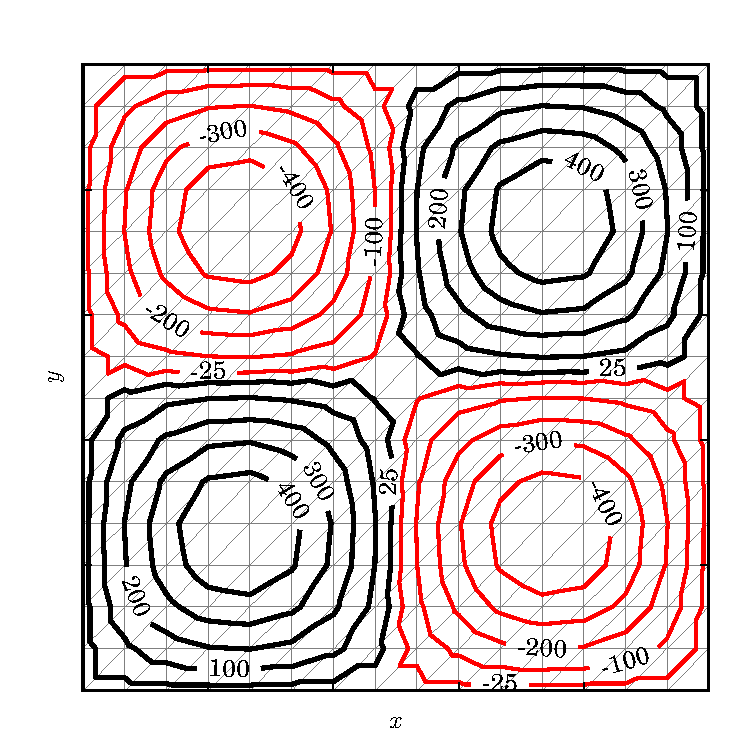
\includegraphics[width=\linewidth]{images/momentum/ISMIP_HOM_A/B.pdf}
  \caption[ISMIP-HOM bedrock topography]{ISMIP-HOM A bedrock topography deviation from the average $\hat{B} = B + \bar{B} - S$ over the $\ell \times \ell$ square km grid.  The \CSLVR script used to generate the figure is shown in Code Listing \ref{ismip_hom_bed_code}.}
  \label{ismip_hom_a_B}
\end{figure}

\section{Plane-strain simulation} \label{ssn_plane_strain_simulation}

\index{Linear differential equations!2D}
\index{Plane-strain simulations}
For an example simulation of the plane-strain model of \S \ref{ssn_plane_strain}, we create a two-dimensional ice-sheet with surface height 
{\small
\begin{align*}
  S(x) = \left( \frac{ H_{max} + B_0 - S_0 }{2} \right) \cos\left( \frac{2\pi}{\ell} x \right) + \left( \frac{H_{max} + B_0 + S_0}{2} \right),
\end{align*}}
with thickness at the divide $H_{max}$, height of terminus above water $S_0$, depth of ice terminus below water $B_0$, and width $\ell$.  We prescribe the sinusoidally-varying basal topography
\begin{align*}
  B(x) = b \cos\left( n_b \frac{2\pi}{\ell} x \right) + B_0,
\end{align*}
with amplitude $b$ and number of bumps $n_b$.  The basal traction field used followed the same sinusoidal variation as the surface,
\begin{align*}
  \beta(x) = \left( \frac{\beta_{max} - \beta_{min}}{2} \right) \cos\left( \frac{2\pi}{\ell} x \right) + \left( \frac{\beta_{max} + \beta_{min}}{2} \right)
\end{align*}
with maximum value $\beta_{max}$ and minimum value $\beta_{min}$.  The specific values used by the simulation are listed in Table \ref{plane_strain_values} with results depicted in Figure \ref{plane_strain_image} generated by Code Listing \ref{plane_strain_momentum_code}.

\begin{table}[H]
\centering
\caption[Plane-strain momentum variables]{Variable values for plane-strain simulation.}
\label{plane_strain_values}
\begin{tabular}{llll}
\hline
\textbf{Variable} & \textbf{Value} & \textbf{Units} & \textbf{Description} \\
\hline
$\dot{\varepsilon}_0$ & $10\sups{-15}$ & a\sups{-1}   & strain regularization \\
$A$       & $10\sups{-16}$  & Pa\sups{-3}a\sups{-1}   & flow-rate factor \\
$F_b$     & $0$             & m a\sups{-1}            & basal water discharge \\
$k_x$     & $150$           & -- & number of $x$ divisions \\
$k_z$     & $10$            & -- & number of $z$ divisions \\
$N_e$     & $3000$          & -- & number of cells \\
$N_n$     & $1661$          & -- & number of vertices \\
$\ell$    & $400$           & km & width of domain \\
$H_{max}$ & $4000$          & m  & thickness at divide \\
$S_0$     & $100$           & m  & terminus height \\
$B_0$     & $-200$          & m  & terminus depth \\
$n_b$     & $25$            & -- & number of bed bumps \\
$b$       & $50$            & m  & bed bump amplitude \\
$\beta_{max}$ & $50$        & kg m\sups{-2}a\sups{-1} & max basal traction \\ 
$\beta_{min}$ & $0.2$       & kg m\sups{-2}a\sups{-1} & min basal traction \\ 
\hline
\end{tabular}
\end{table}

\pythonexternal[label=ismip_hom_bed_code, caption={\CSLVR script used to generate ISMIP-HOM basal topography Figure \ref{ismip_hom_a_B}.}]{scripts/momentum/ISMIP_HOM_A/plot_bed.py}

\pythonexternal[label=ismip_hom_momentum_code, caption={\CSLVR script which solves the ISMIP-HOM experiment of \S \ref{ssn_ismip_hom_test_simulations}.}]{scripts/momentum/ISMIP_HOM_A/xsmall/ISMIP_HOM_A_BP.py}

\pythonexternal[label=plane_strain_momentum_code, caption={\CSLVR source code used to solve the plane-strain problem of \S \ref{ssn_plane_strain_simulation}.}]{scripts/momentum/plane_strain/plane_strain.py}
\begin{figure*}
  \centering
    
    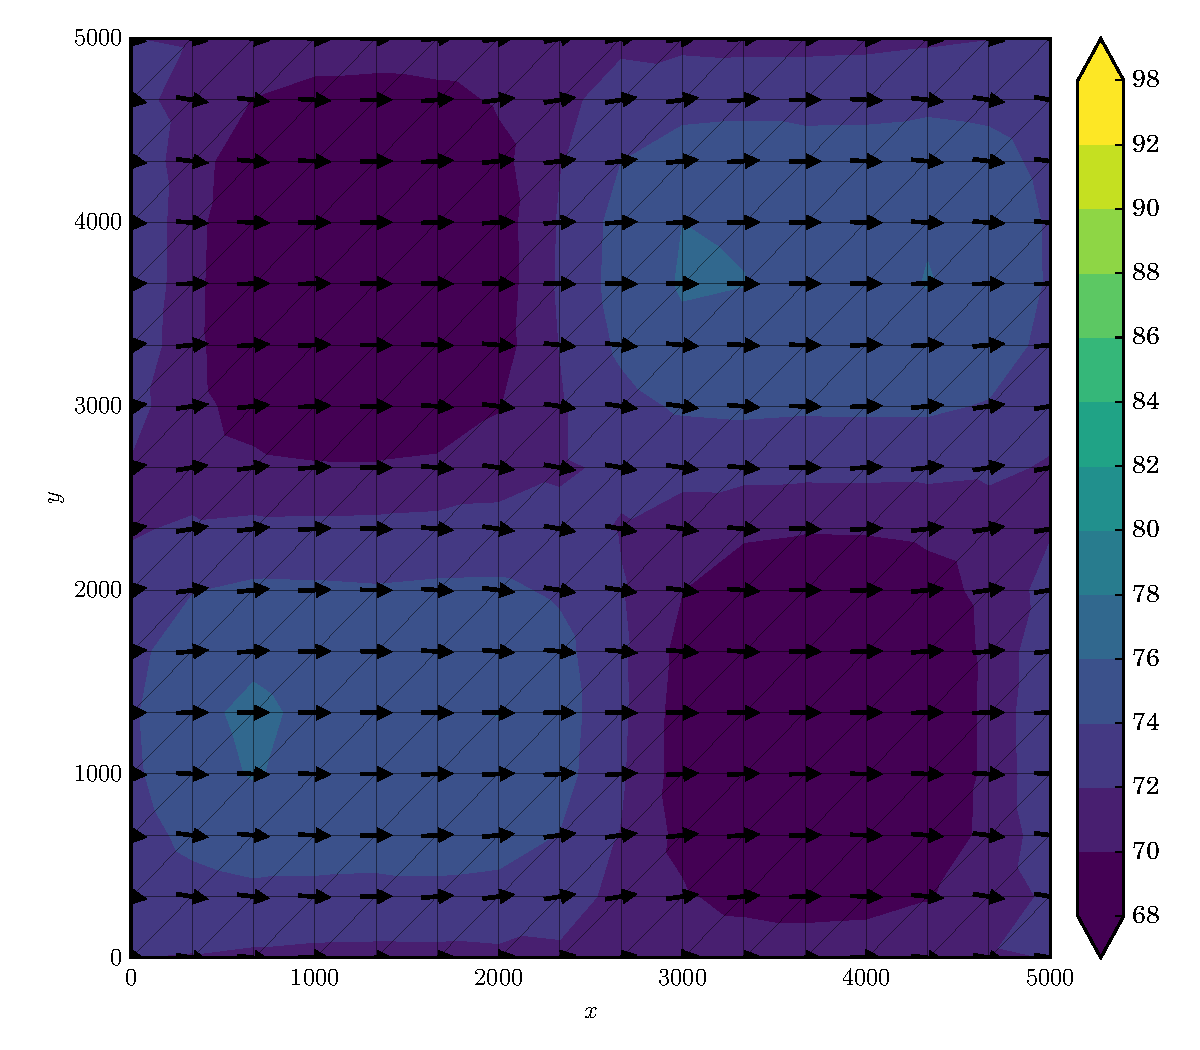
\includegraphics[width=0.3\linewidth]{images/momentum/ISMIP_HOM_A/xsmall/FS/U_mag.pdf}
    \quad
    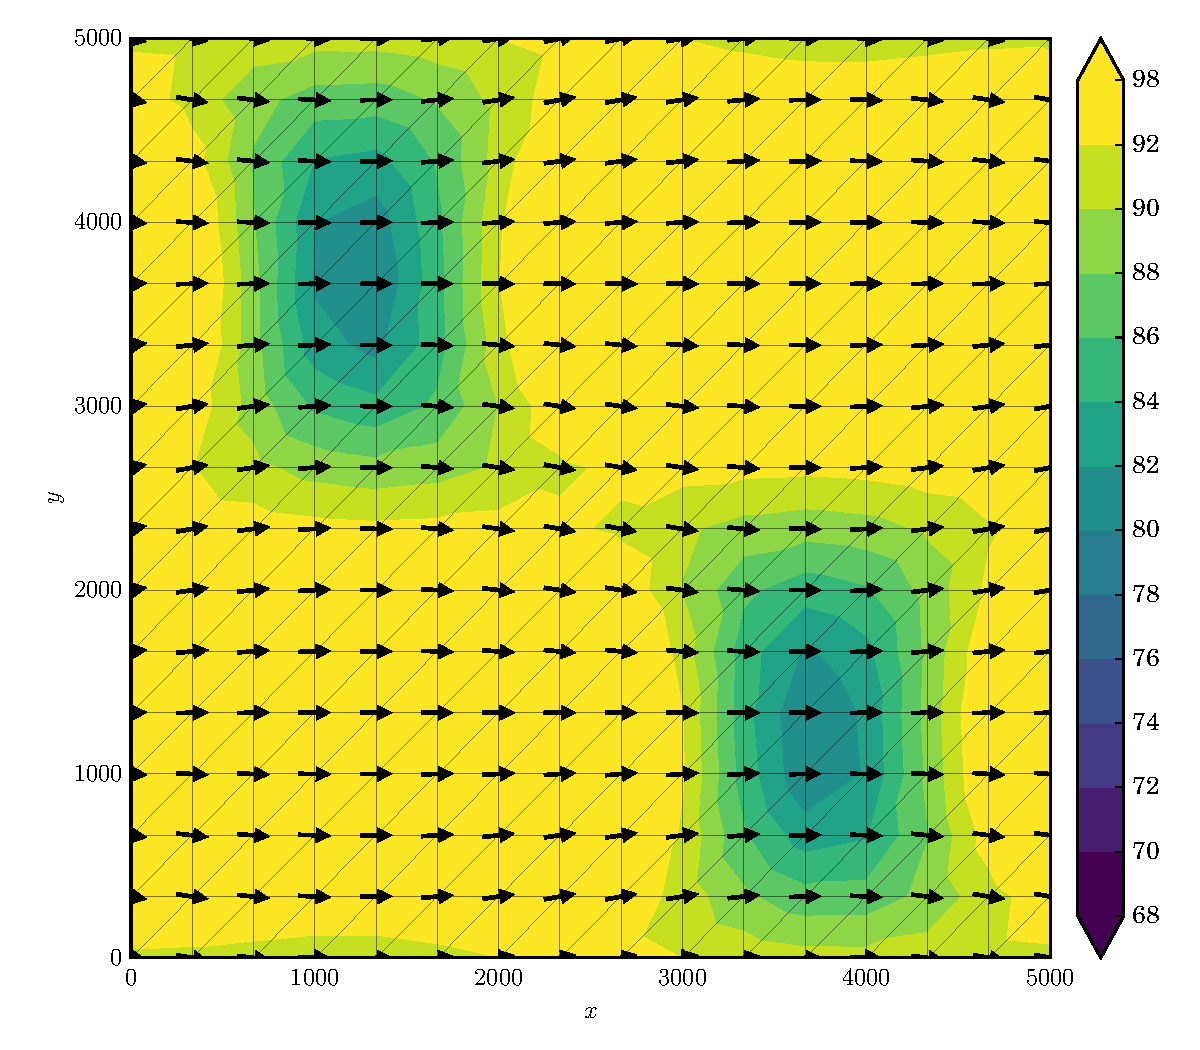
\includegraphics[width=0.3\linewidth]{images/momentum/ISMIP_HOM_A/xsmall/RS/U_mag.pdf}
    \quad
    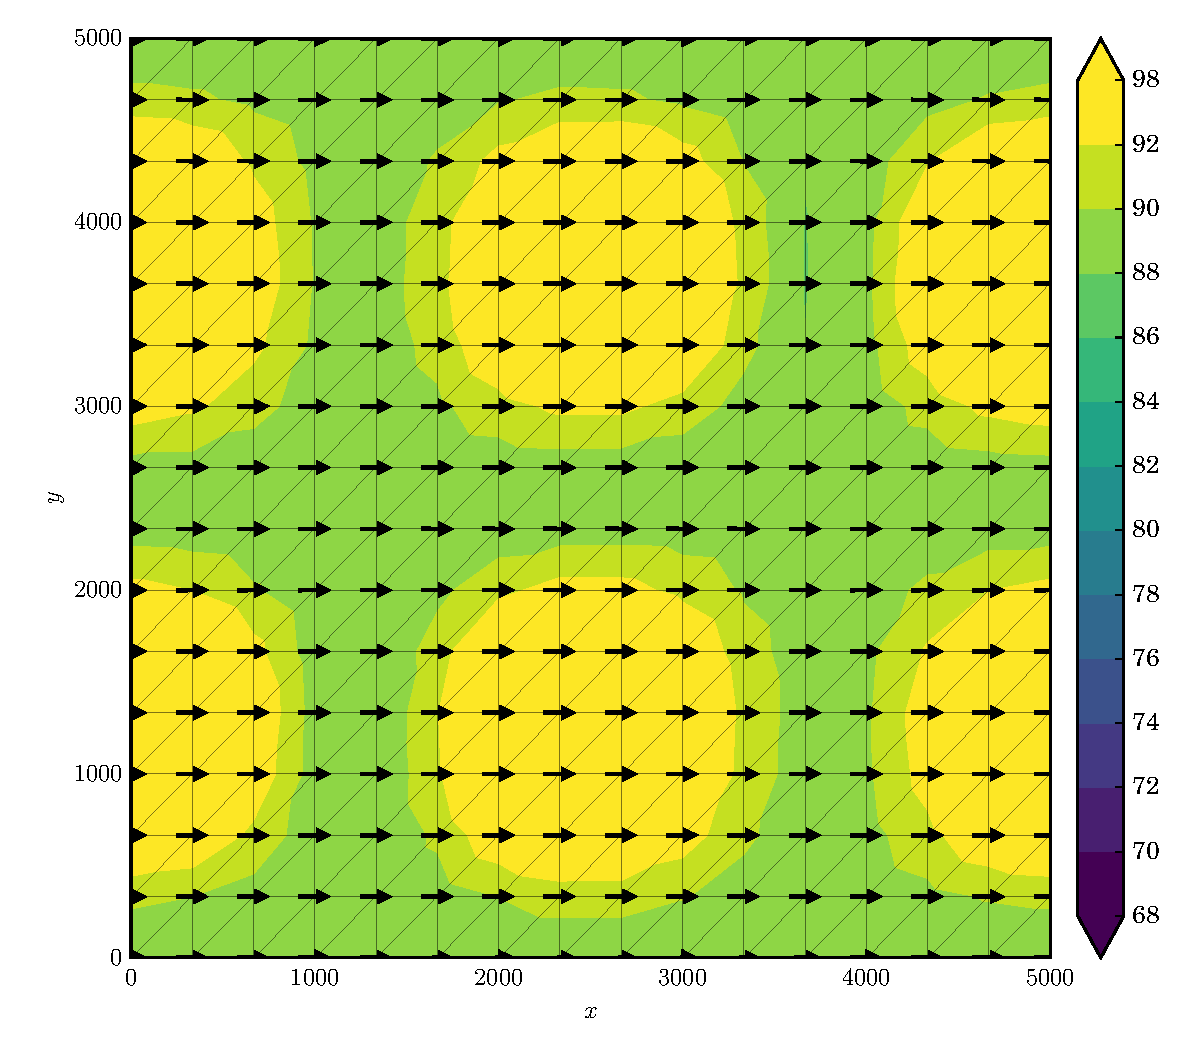
\includegraphics[width=0.3\linewidth]{images/momentum/ISMIP_HOM_A/xsmall/BP/U_mag.pdf}

    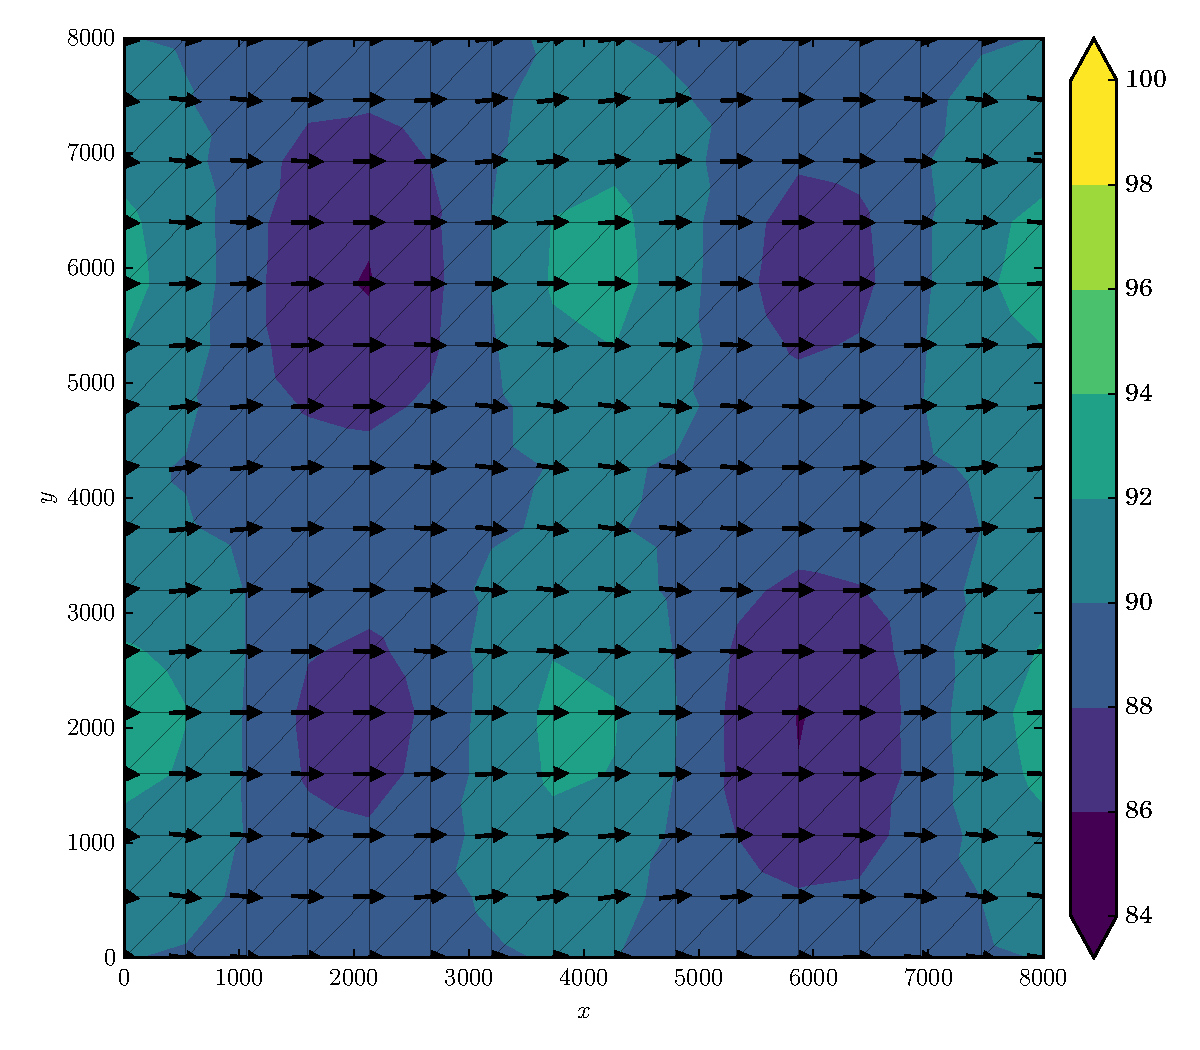
\includegraphics[width=0.3\linewidth]{images/momentum/ISMIP_HOM_A/small/FS/U_mag.pdf}
    \quad
    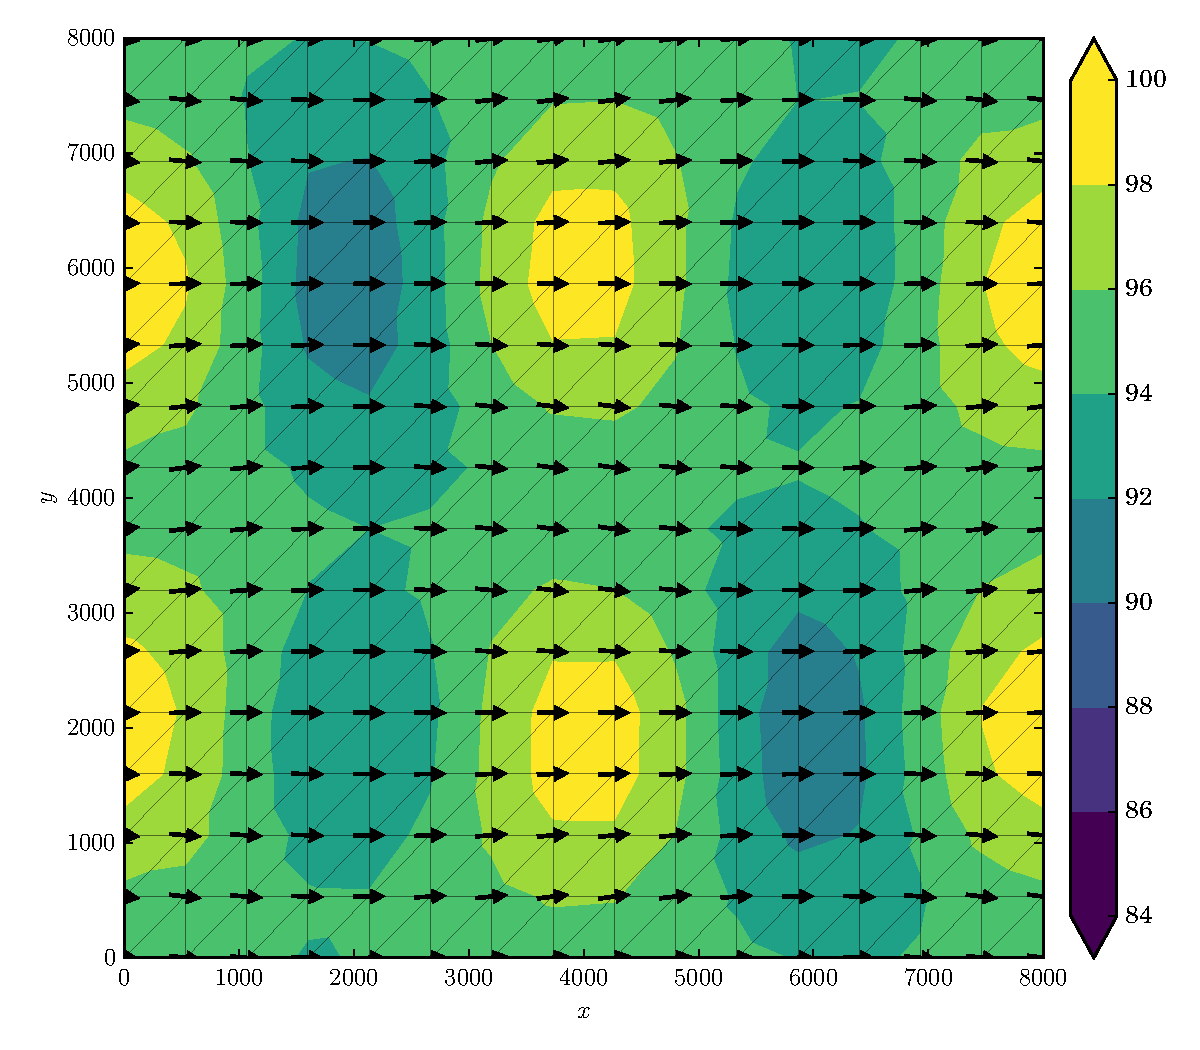
\includegraphics[width=0.3\linewidth]{images/momentum/ISMIP_HOM_A/small/RS/U_mag.pdf}
    \quad
    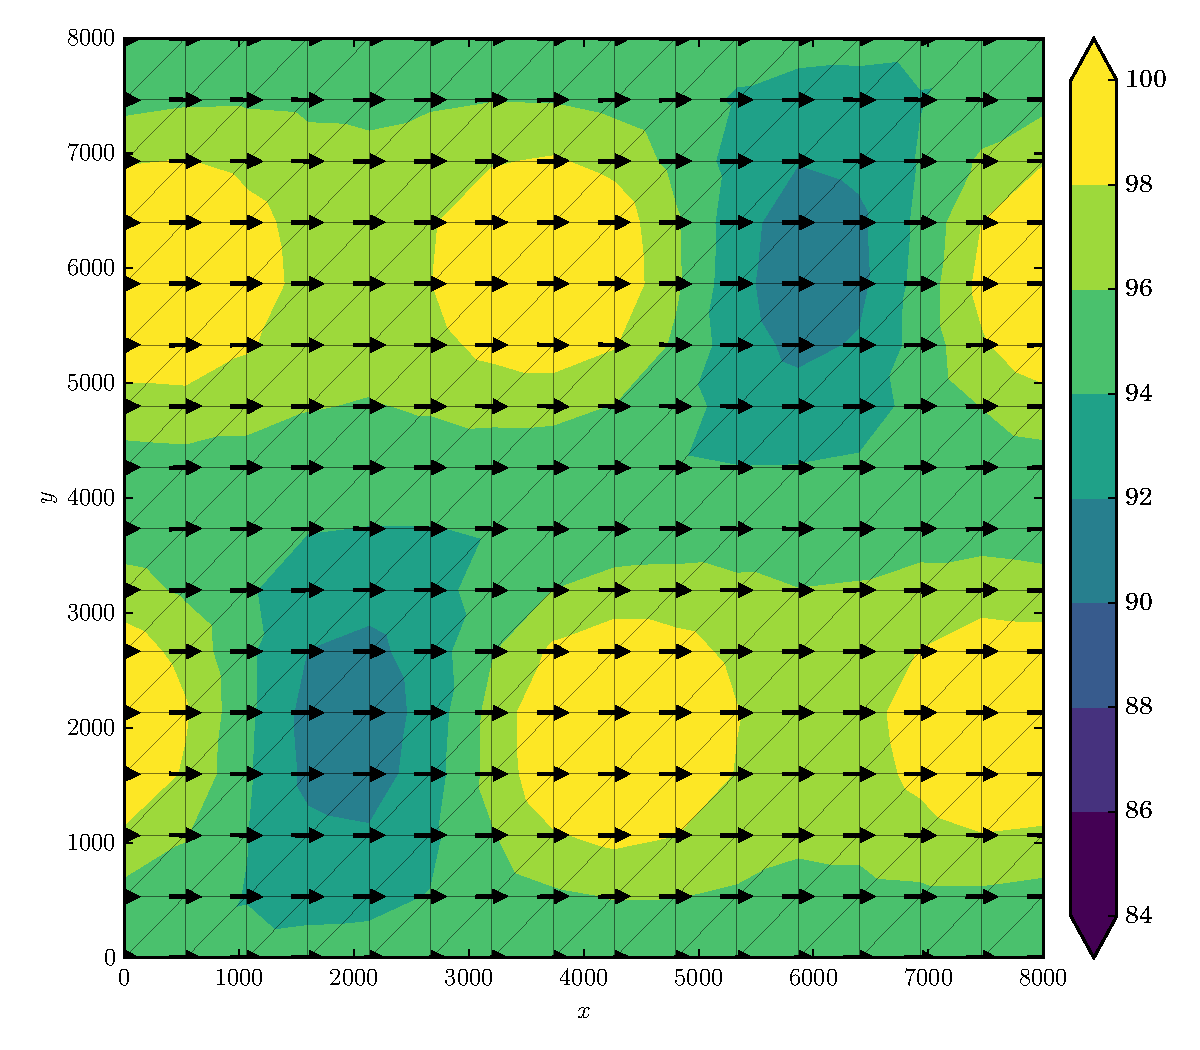
\includegraphics[width=0.3\linewidth]{images/momentum/ISMIP_HOM_A/small/BP/U_mag.pdf}

    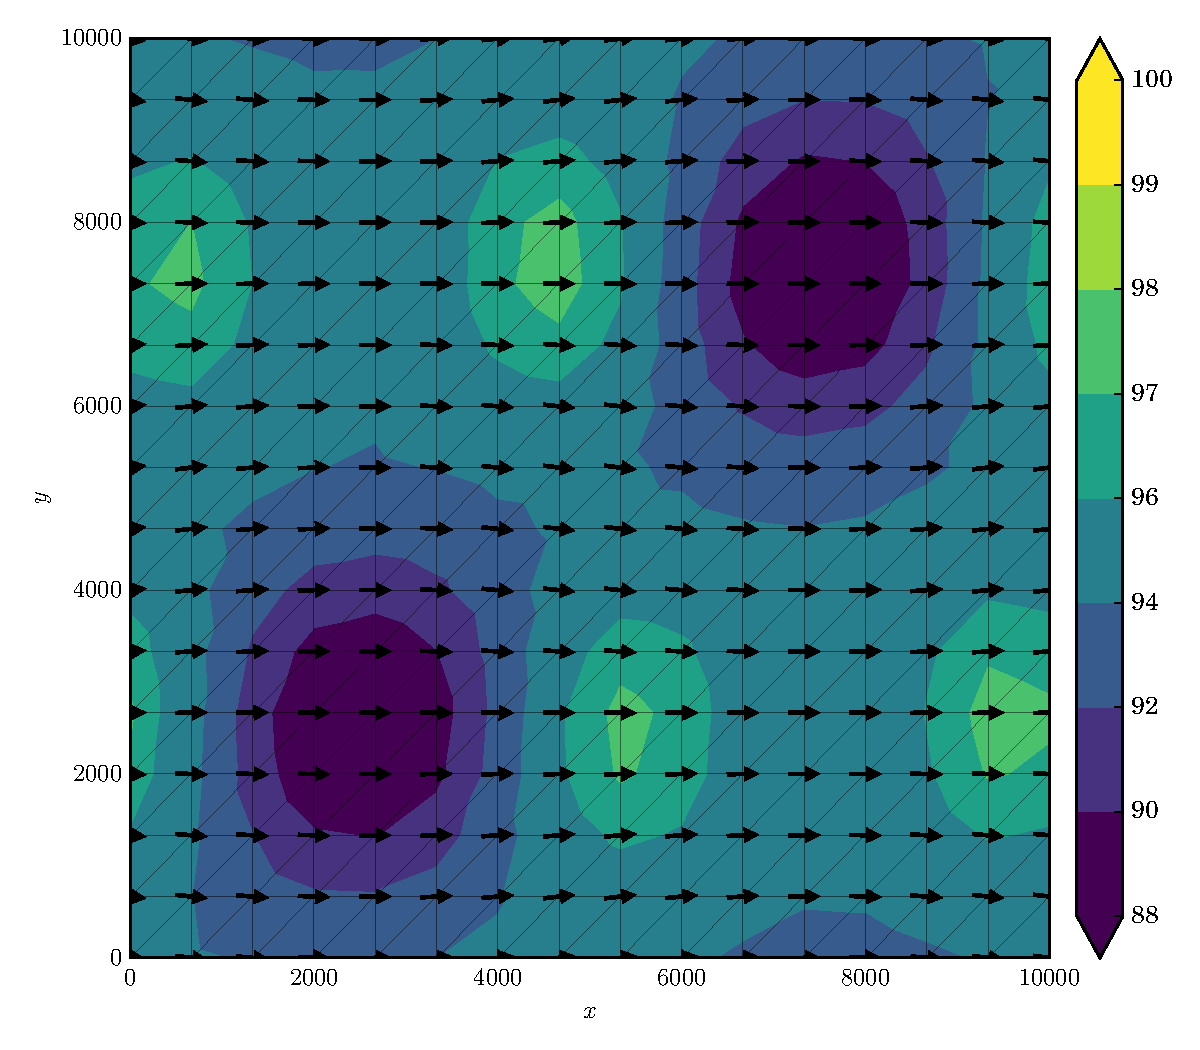
\includegraphics[width=0.3\linewidth]{images/momentum/ISMIP_HOM_A/medium/FS/U_mag.pdf}
    \quad
    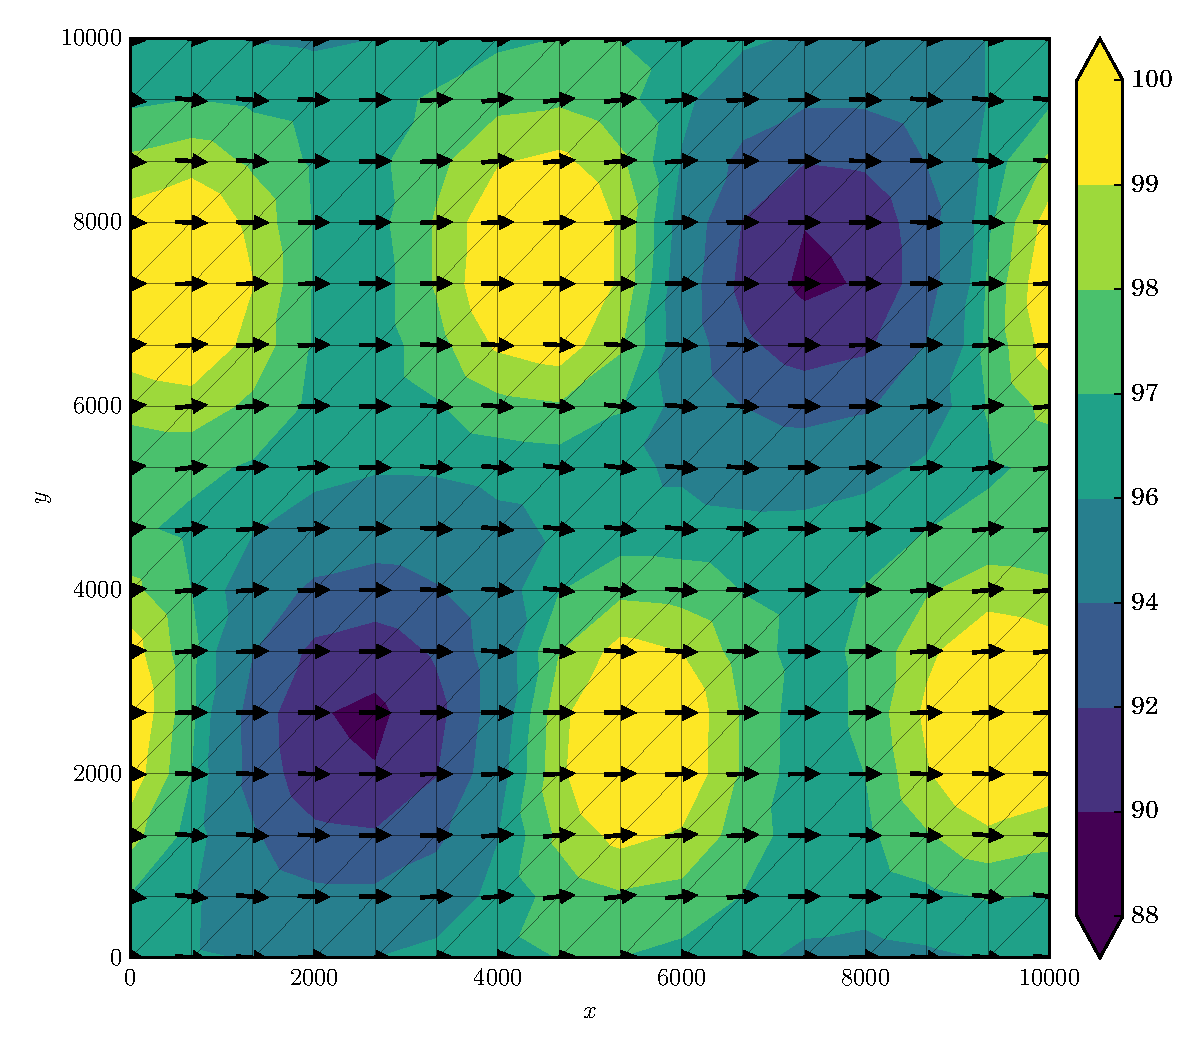
\includegraphics[width=0.3\linewidth]{images/momentum/ISMIP_HOM_A/medium/RS/U_mag.pdf}
    \quad
    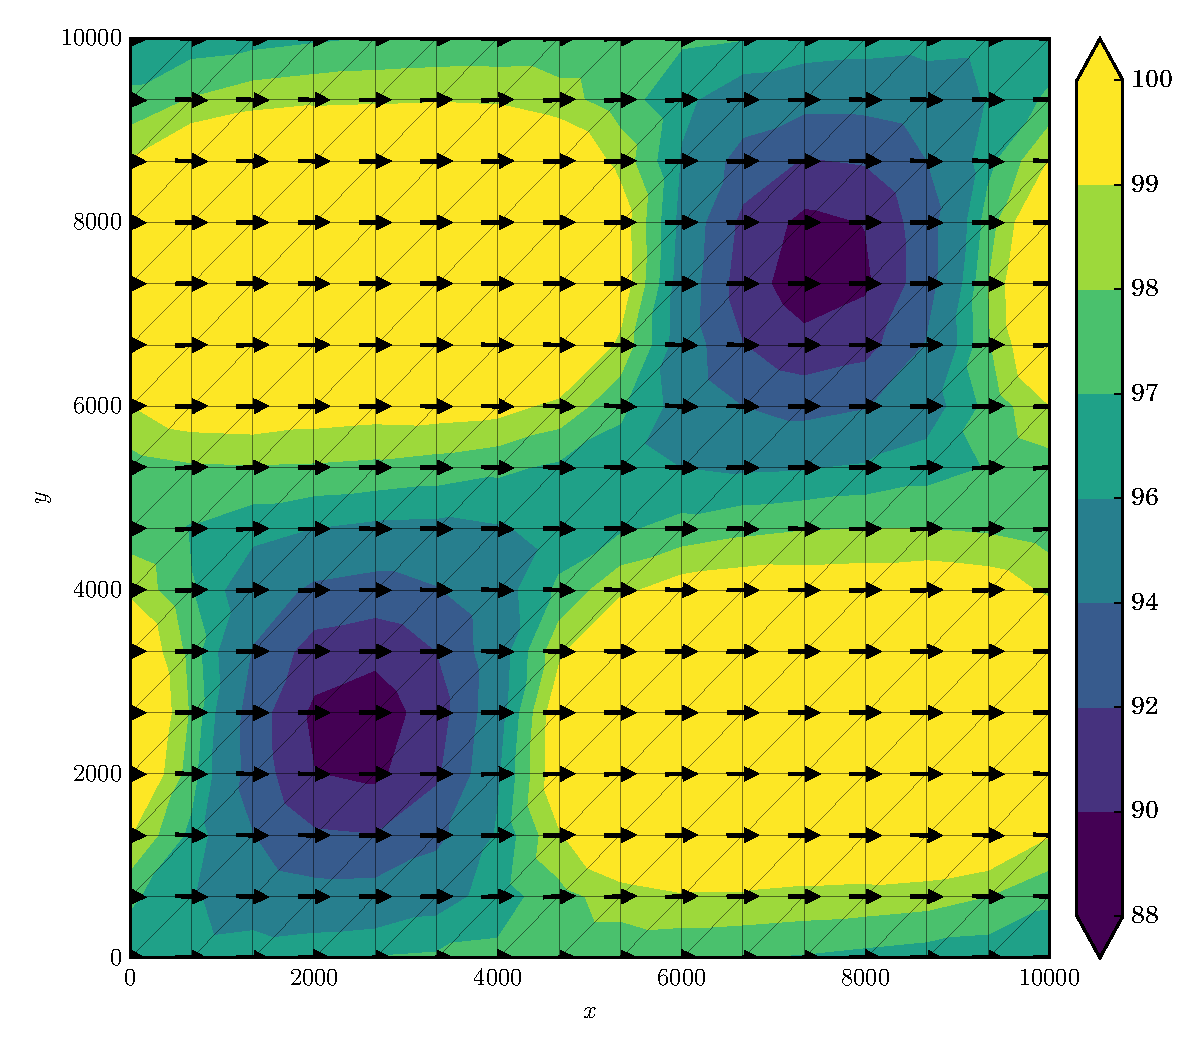
\includegraphics[width=0.3\linewidth]{images/momentum/ISMIP_HOM_A/medium/BP/U_mag.pdf}

    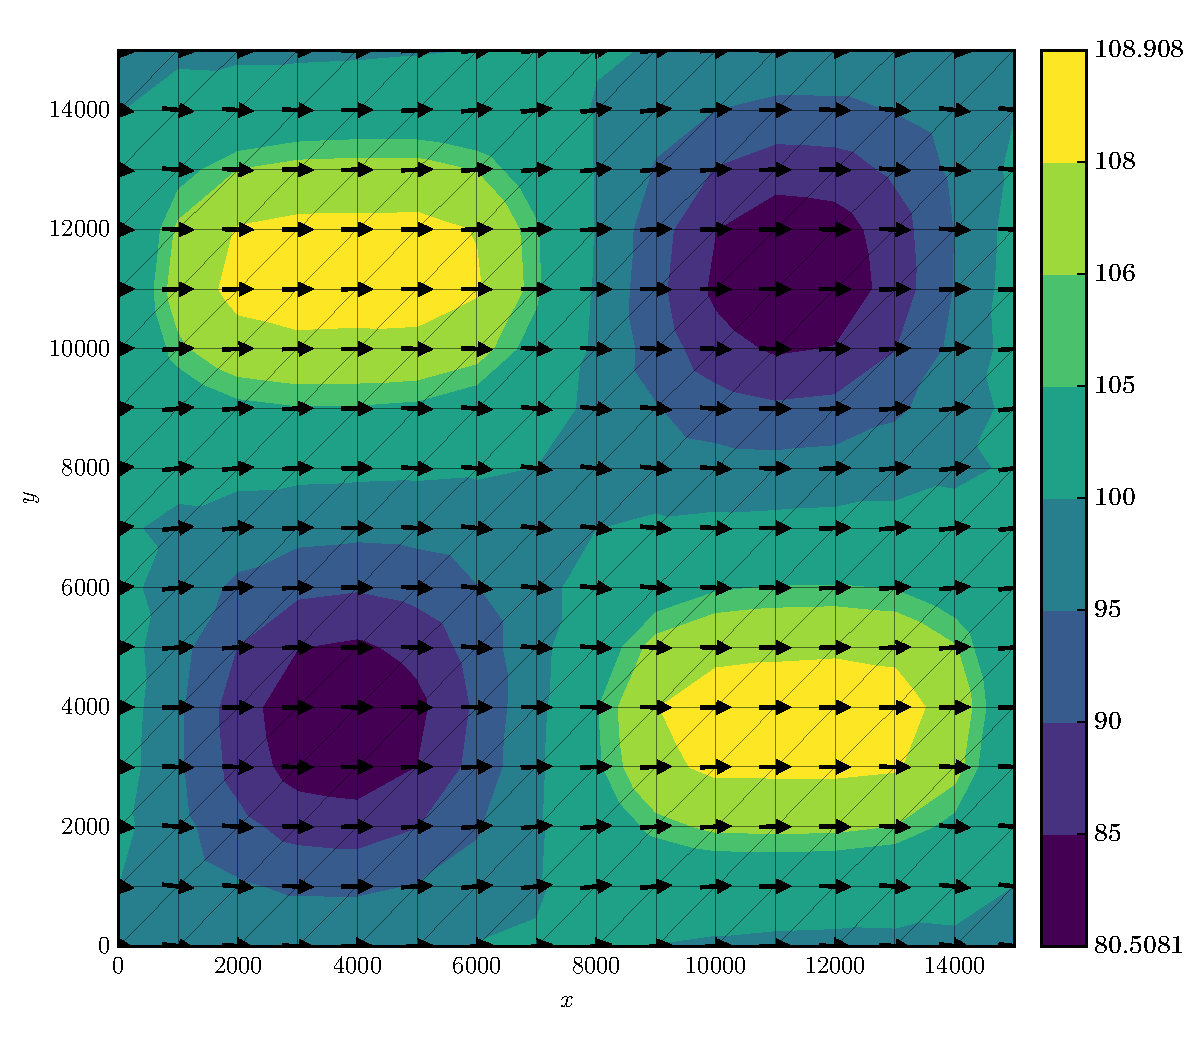
\includegraphics[width=0.3\linewidth]{images/momentum/ISMIP_HOM_A/large/FS/U_mag.pdf}
    \quad
    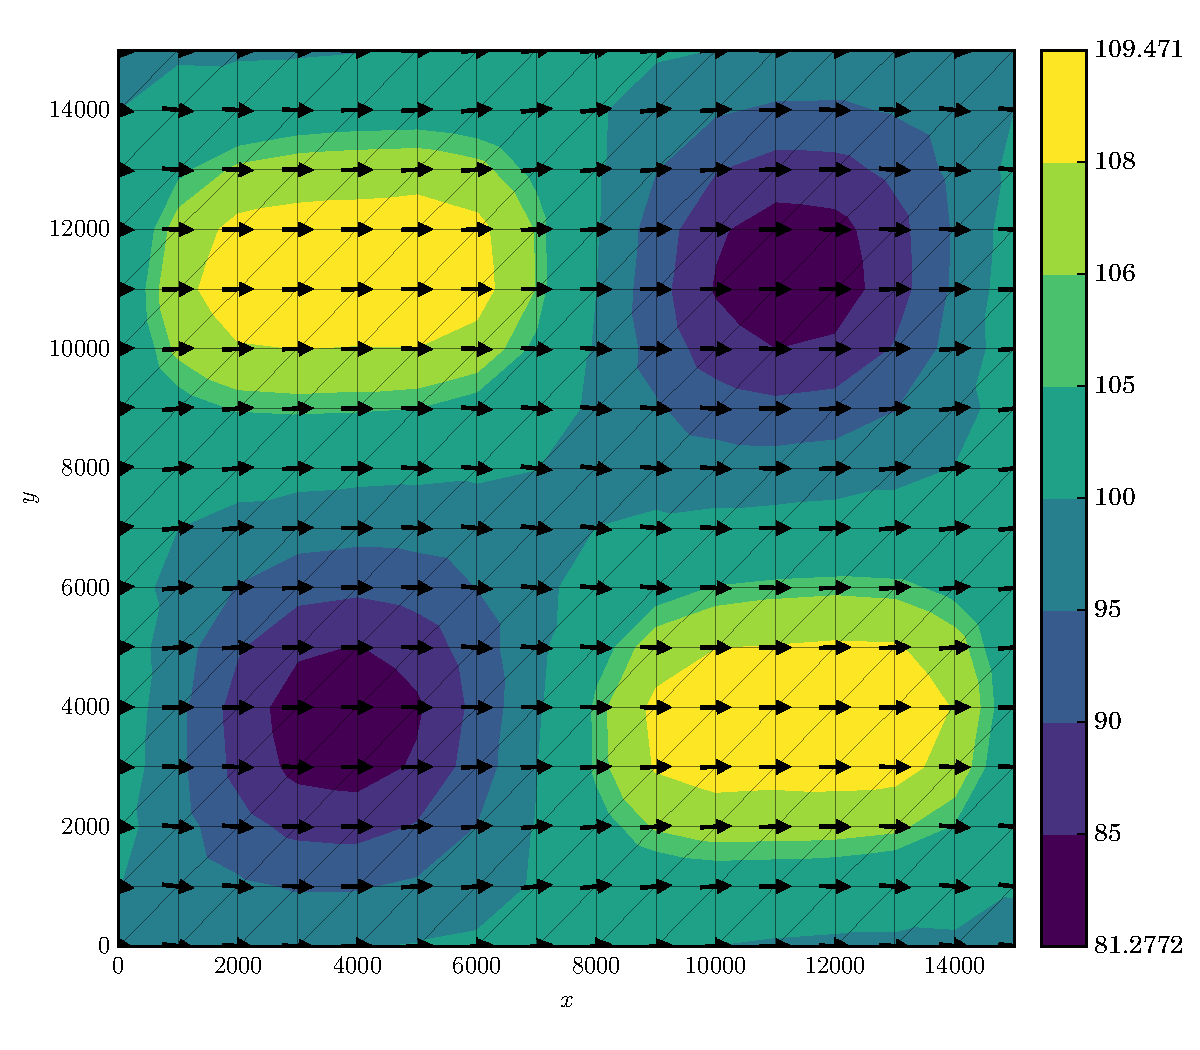
\includegraphics[width=0.3\linewidth]{images/momentum/ISMIP_HOM_A/large/RS/U_mag.pdf}
    \quad
    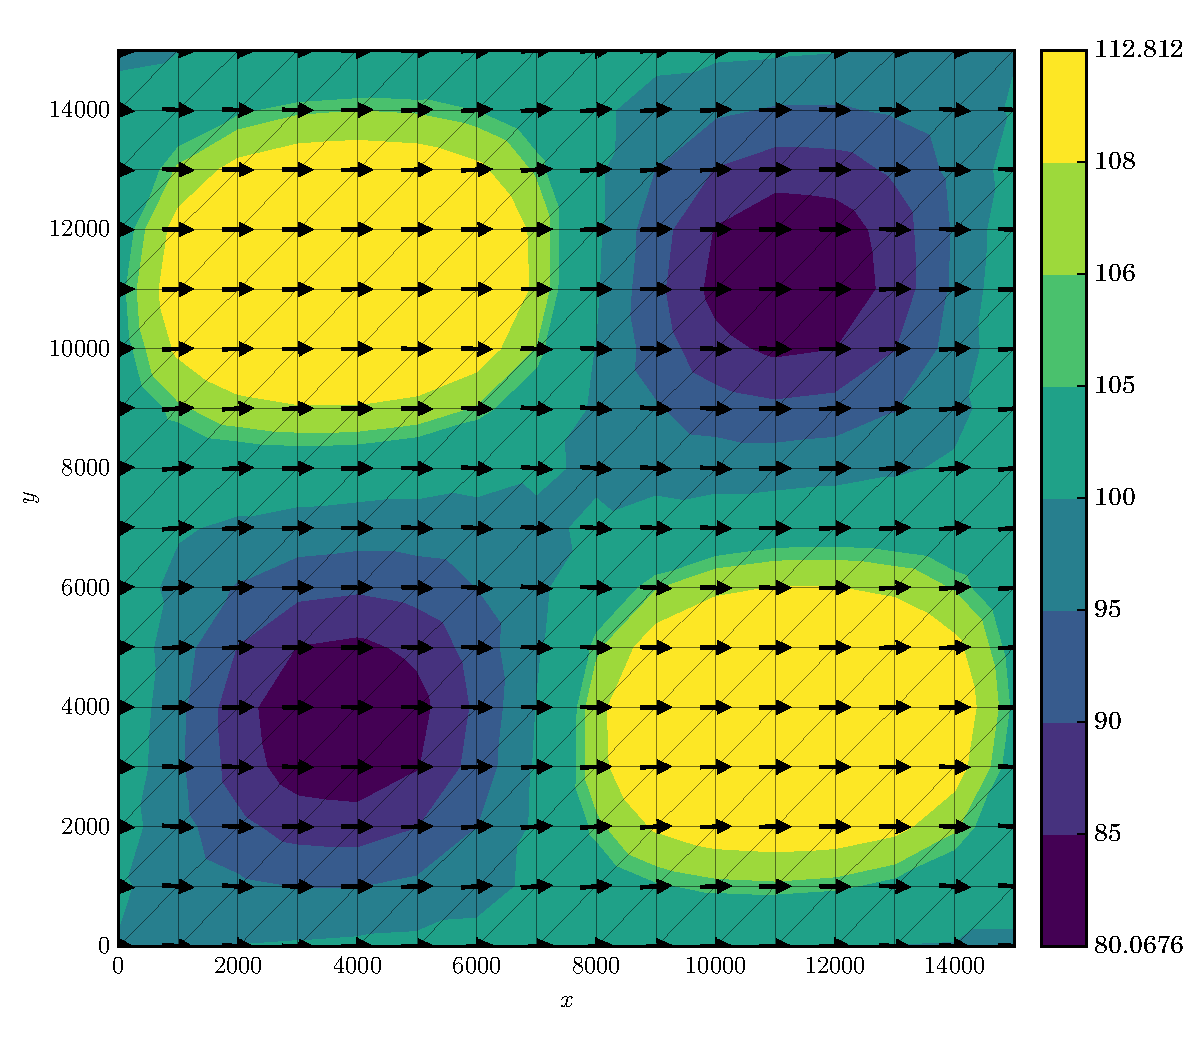
\includegraphics[width=0.3\linewidth]{images/momentum/ISMIP_HOM_A/large/BP/U_mag.pdf}

  \caption[ISMIP-HOM momentum experiment velocities]{Surface velocity $\rankone{u}_S$ for the ISMIP-HOM test experiment using a $5 \times 5$ square km grid (first row), $8 \times 8$ km$^2$ grid (second row), $10 \times 10$ km$^2$ grid (third row), and $15 \times 15$ km$^2$ grid (fourth row).  The left column are results obtained using the full-Stokes model from \S \ref{ssn_full_stokes}, the middle column using the reformulated-Stokes model of \S \ref{ssn_reformulated_stokes}, and the right column was generated using the first-order model from \S \ref{ssn_first_order}. The color scale across each column is made identical for ease of comparison. \newline}
  \label{ismip_hom_a_velocity}
\end{figure*}

\begin{figure*}
  \centering

    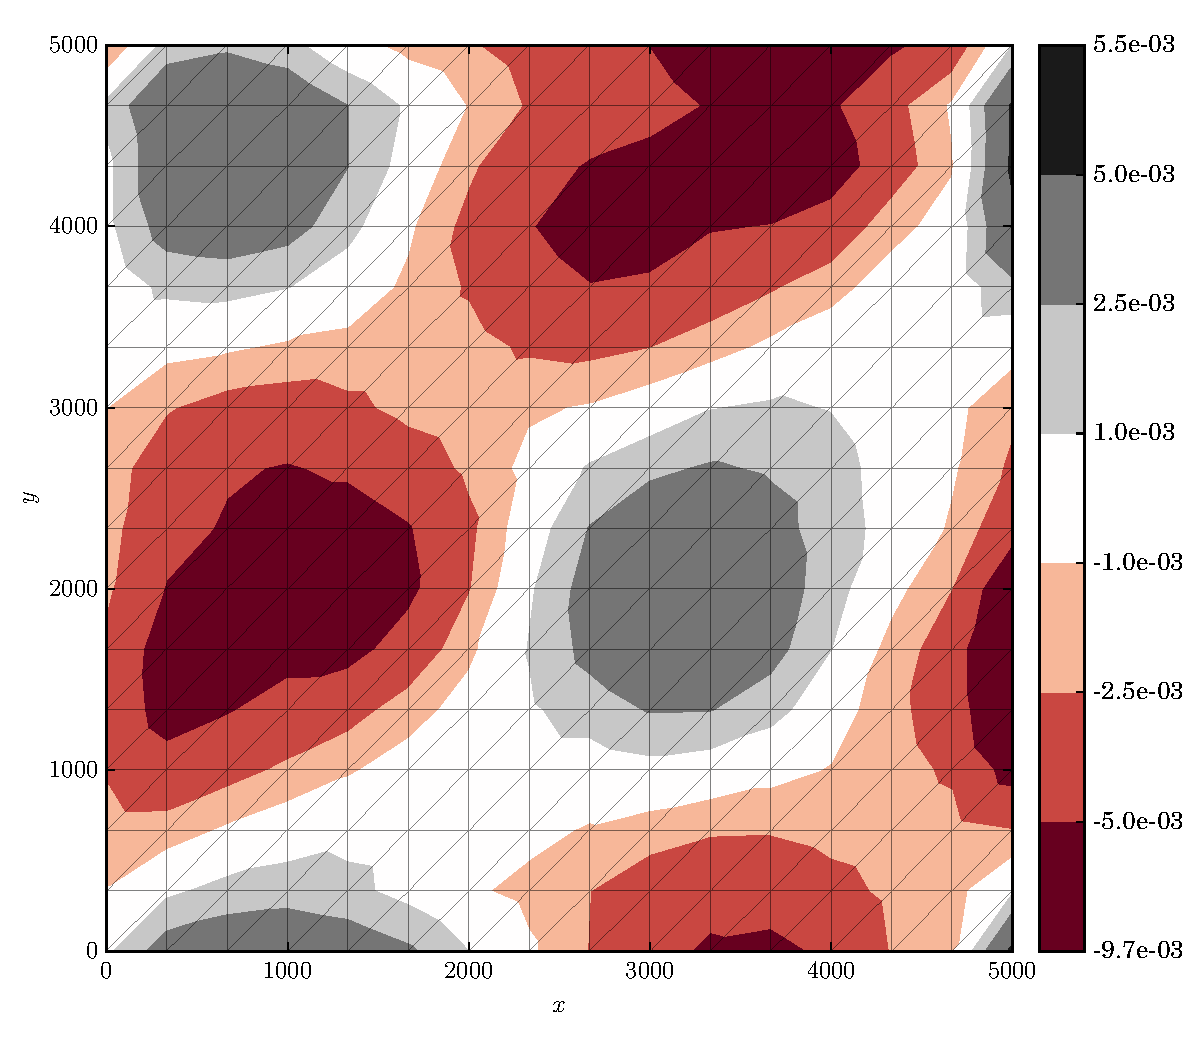
\includegraphics[width=0.3\linewidth]{images/momentum/ISMIP_HOM_A/xsmall/FS/divU.pdf}
    \quad                                           
    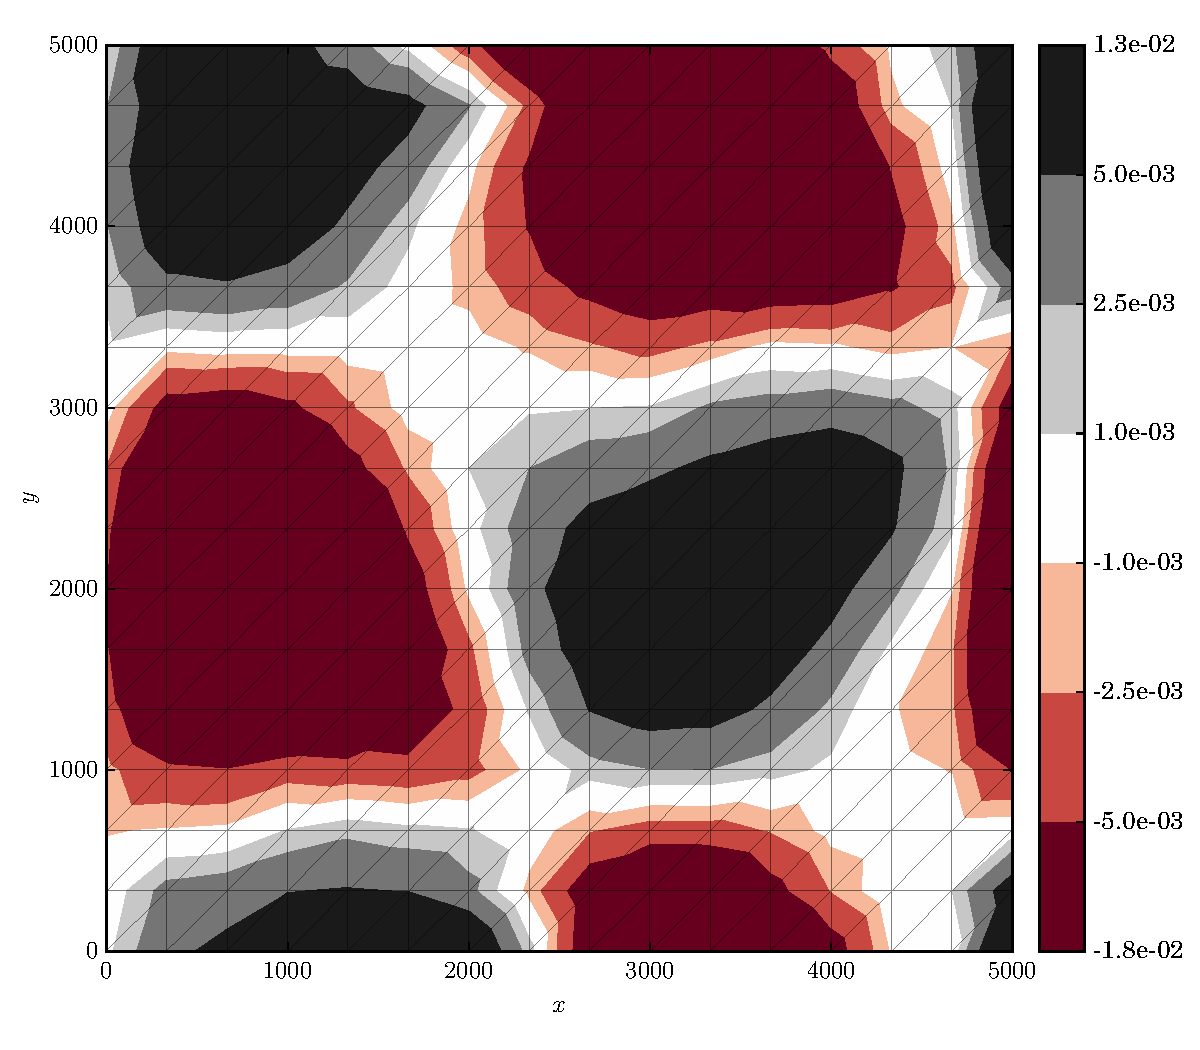
\includegraphics[width=0.3\linewidth]{images/momentum/ISMIP_HOM_A/xsmall/RS/divU.pdf}
    \quad                                           
    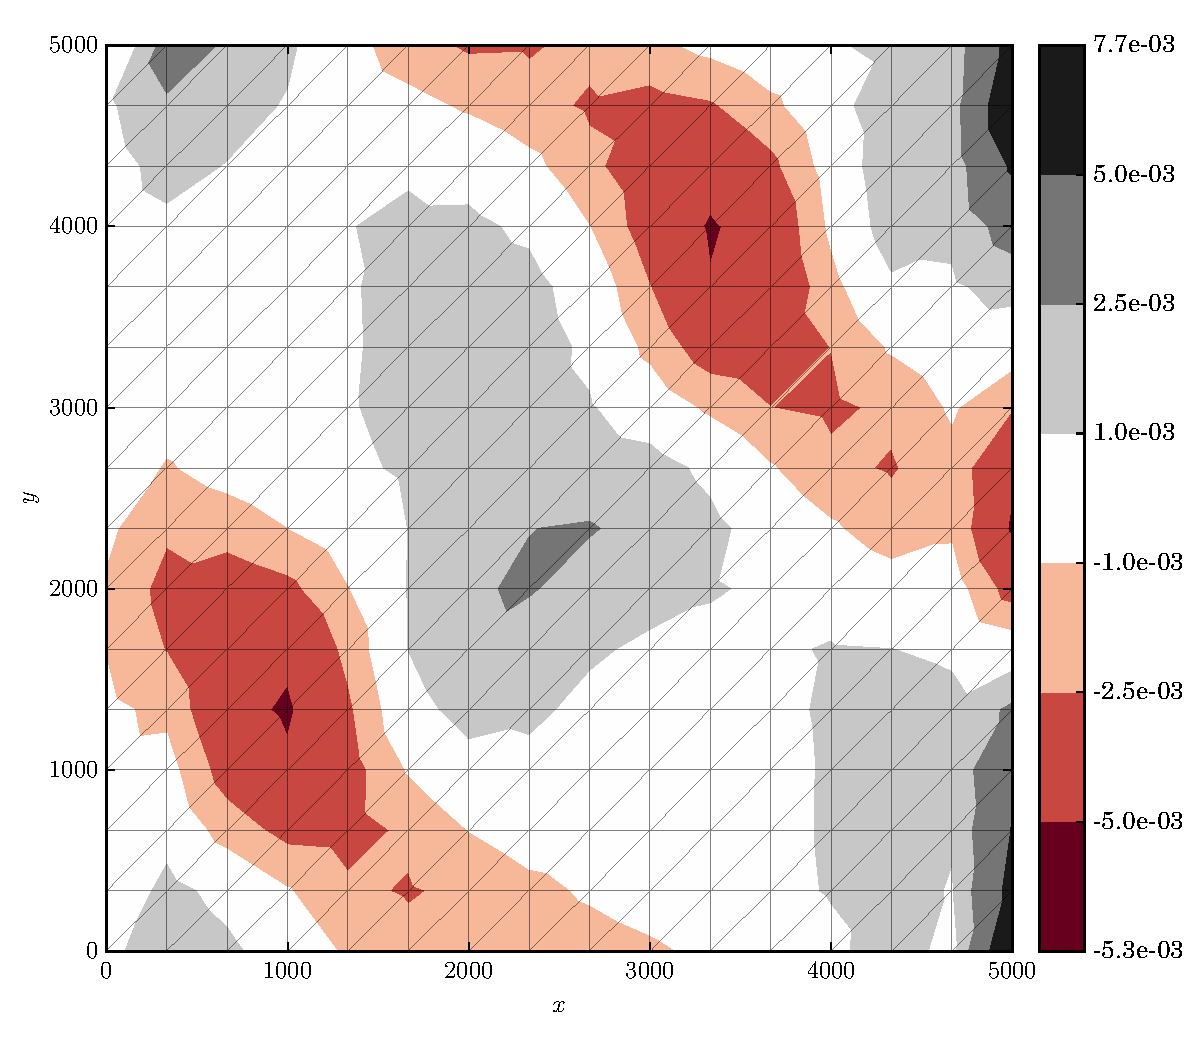
\includegraphics[width=0.3\linewidth]{images/momentum/ISMIP_HOM_A/xsmall/BP/divU.pdf}
                                                    
    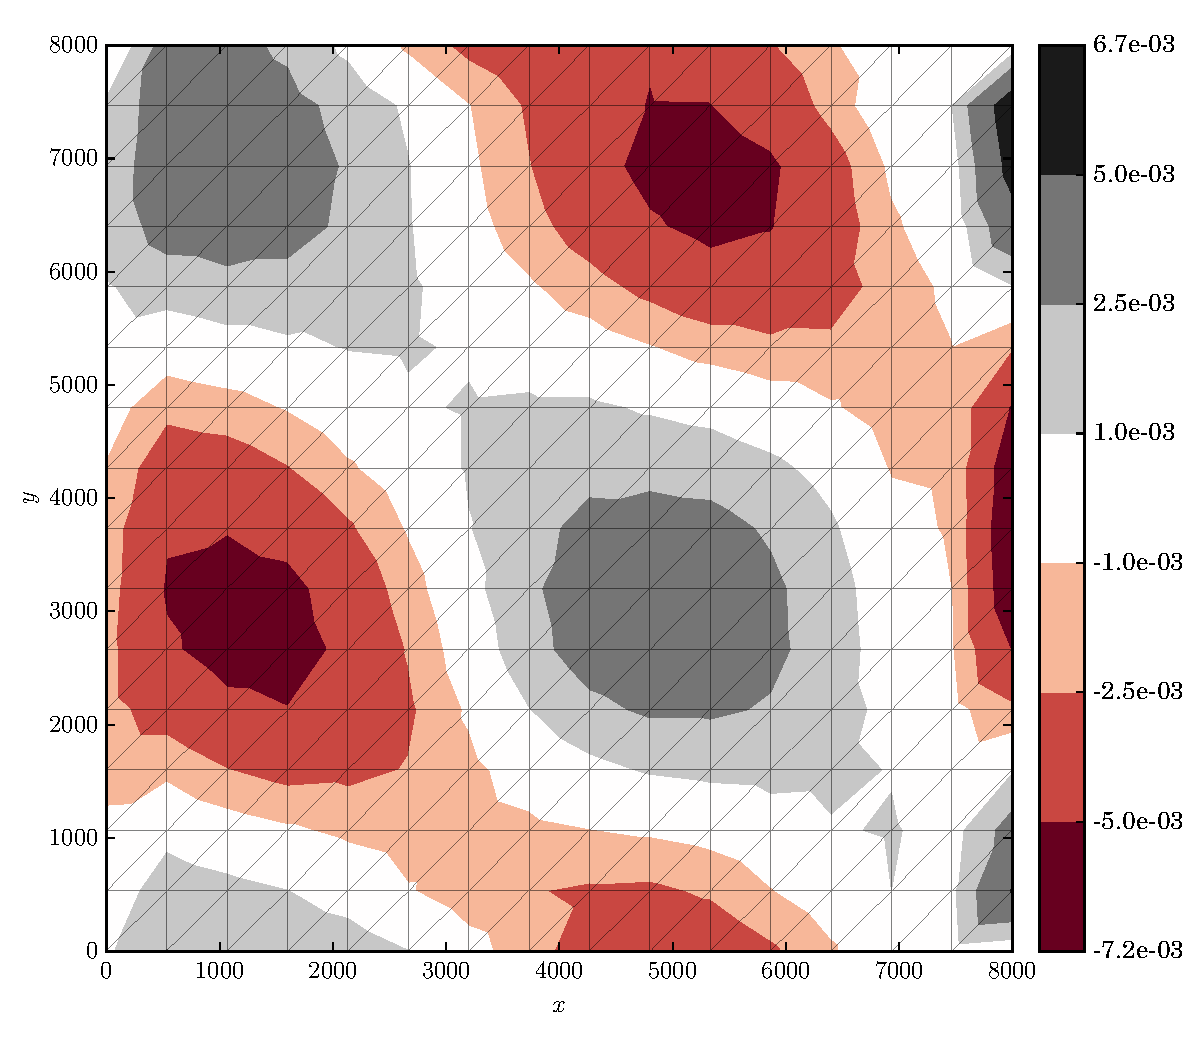
\includegraphics[width=0.3\linewidth]{images/momentum/ISMIP_HOM_A/small/FS/divU.pdf}
    \quad                                           
    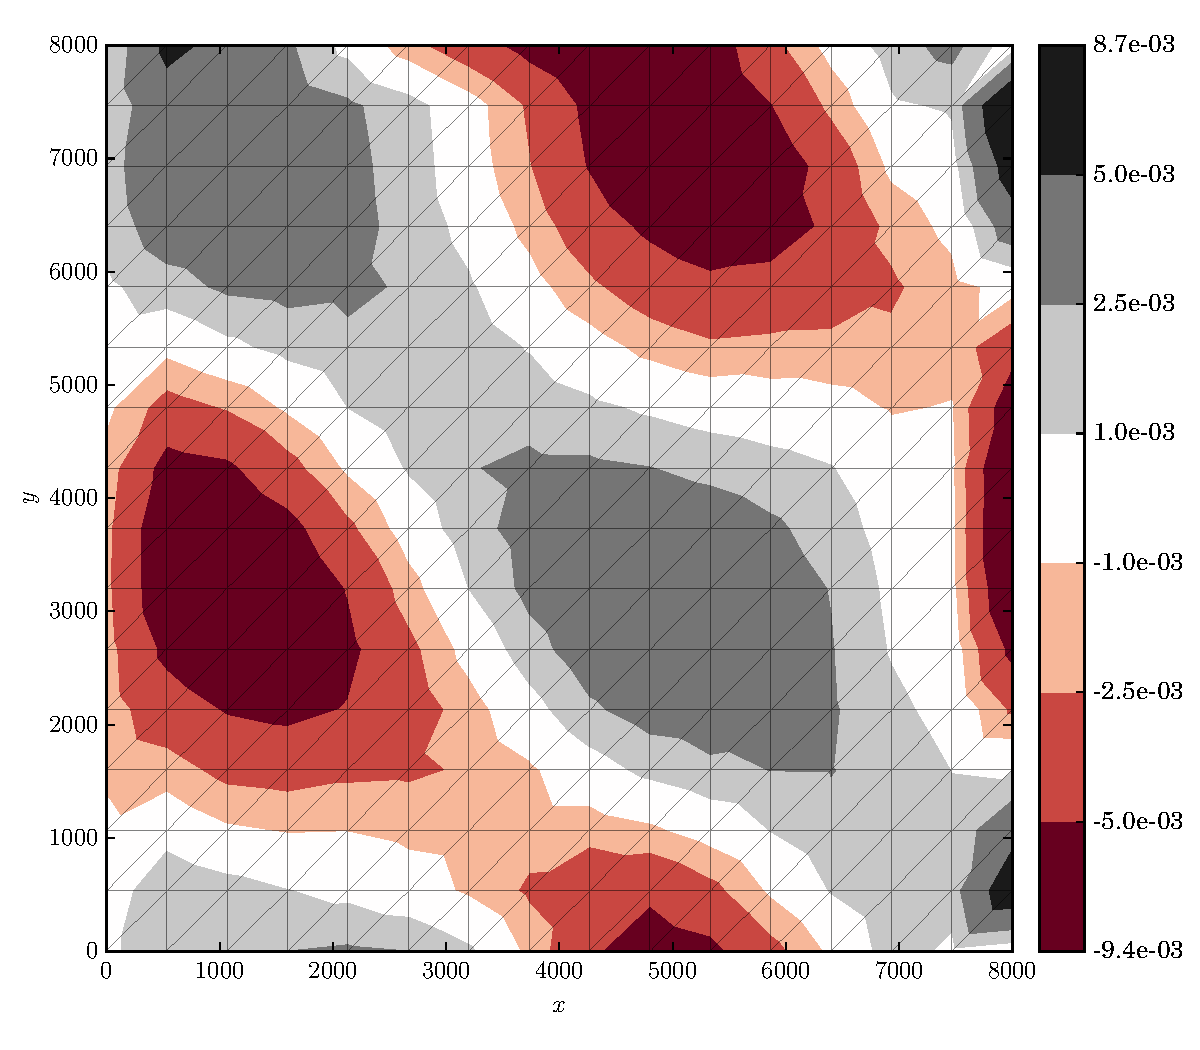
\includegraphics[width=0.3\linewidth]{images/momentum/ISMIP_HOM_A/small/RS/divU.pdf}
    \quad                                           
    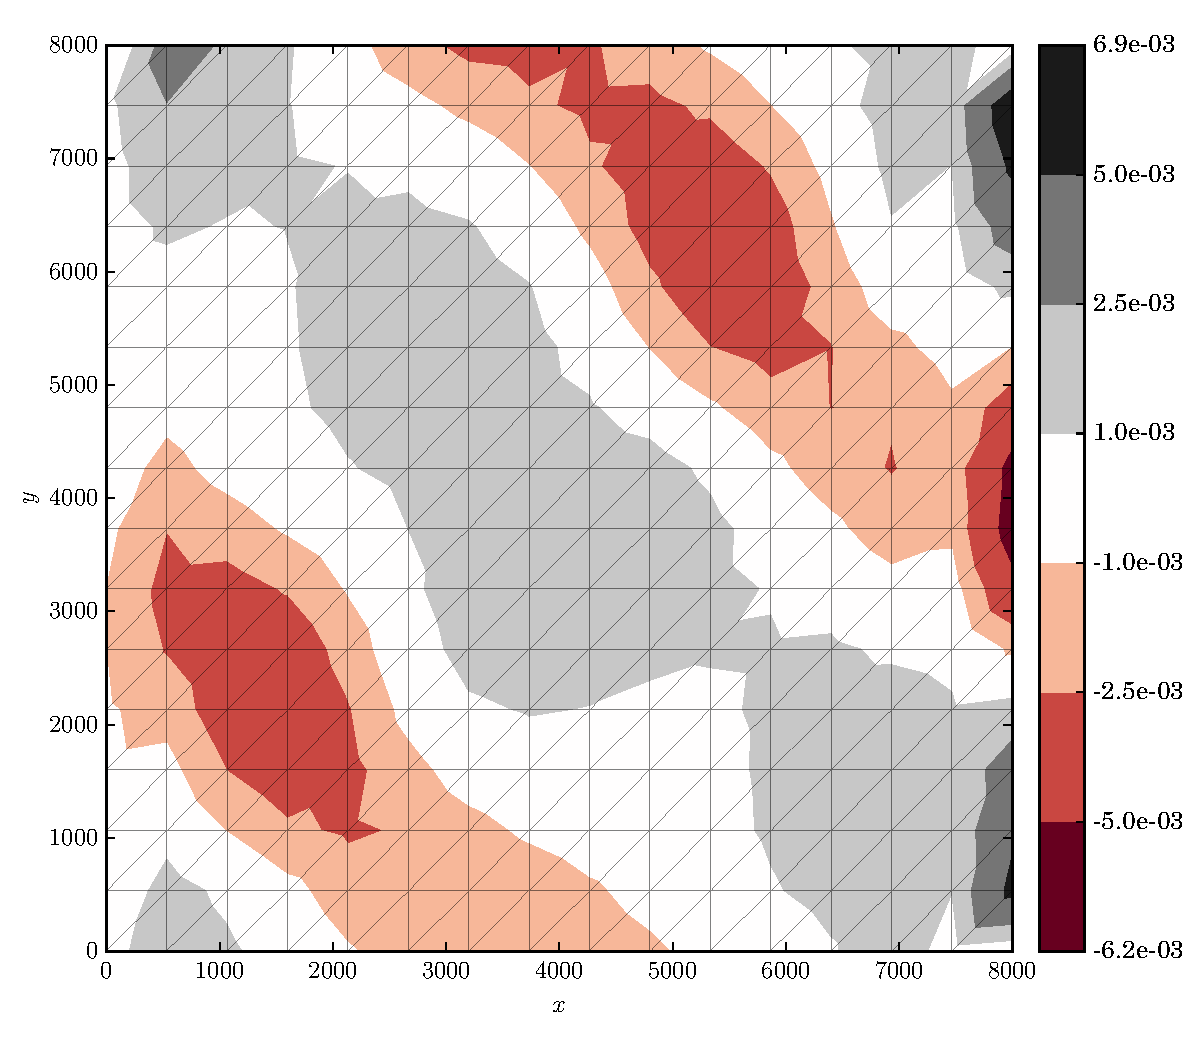
\includegraphics[width=0.3\linewidth]{images/momentum/ISMIP_HOM_A/small/BP/divU.pdf}
                                                    
    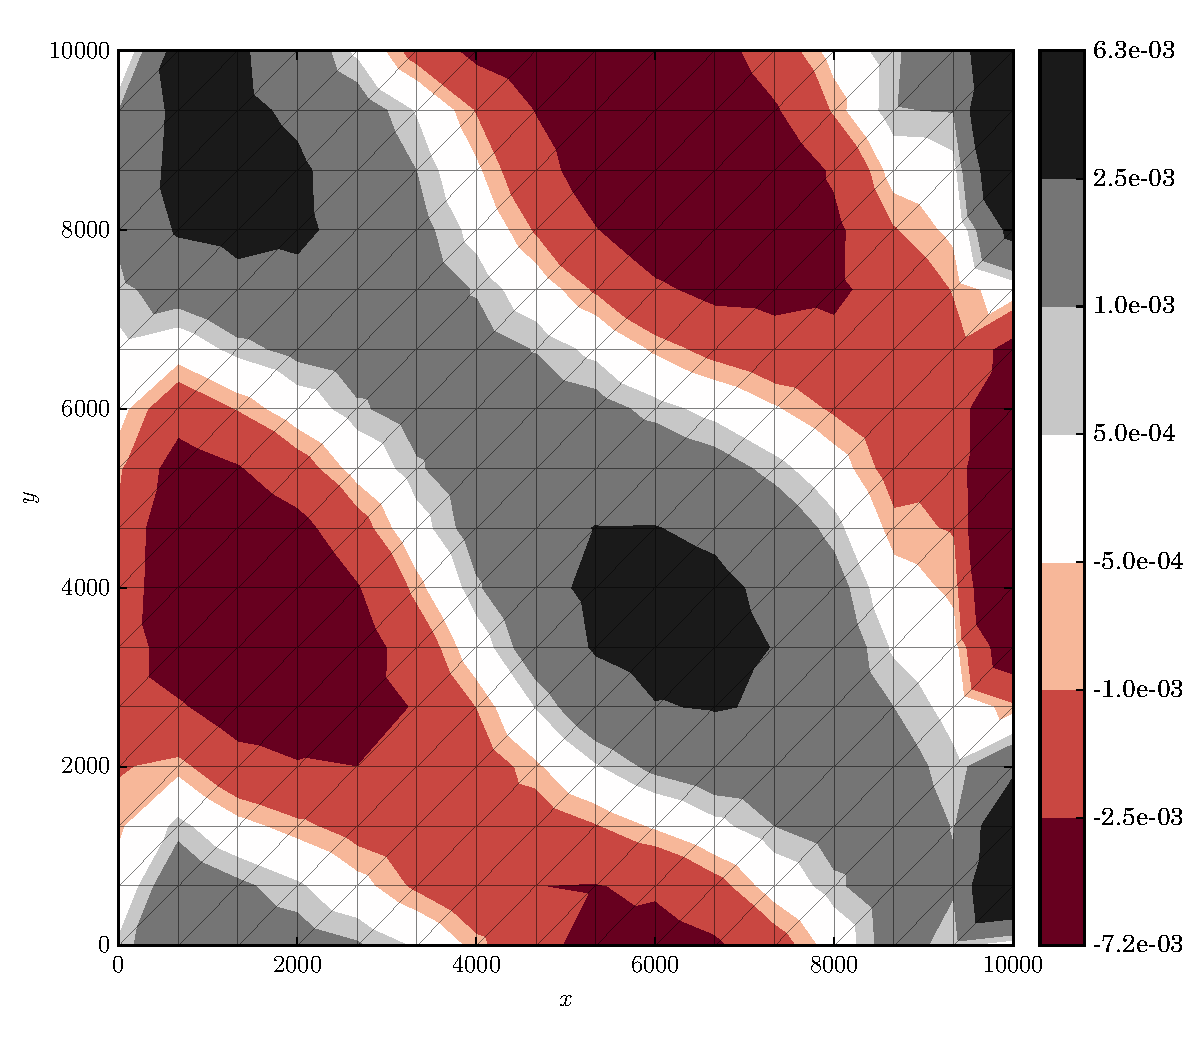
\includegraphics[width=0.3\linewidth]{images/momentum/ISMIP_HOM_A/medium/FS/divU.pdf}
    \quad                                           
    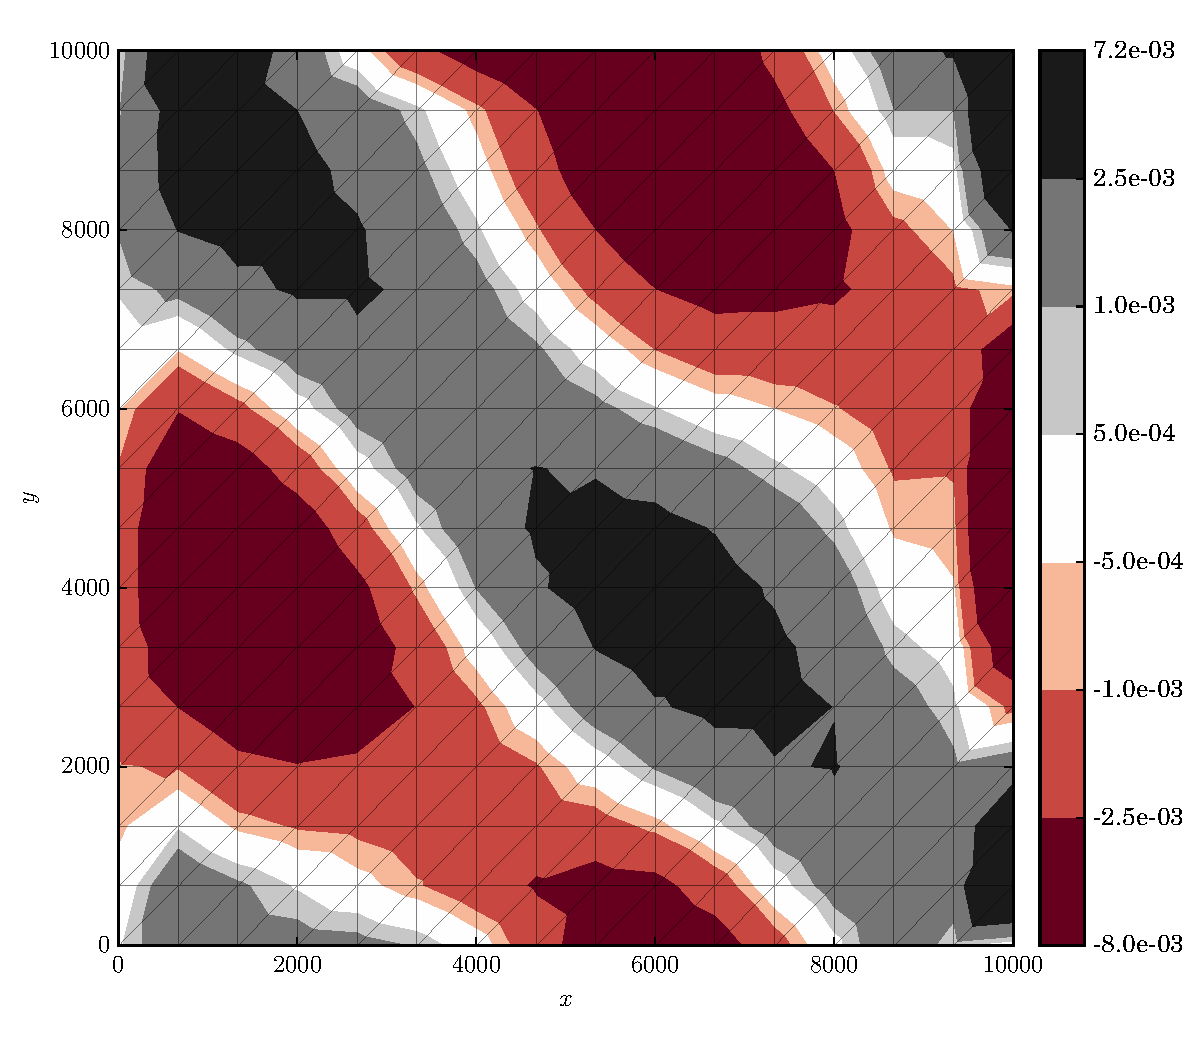
\includegraphics[width=0.3\linewidth]{images/momentum/ISMIP_HOM_A/medium/RS/divU.pdf}
    \quad                                           
    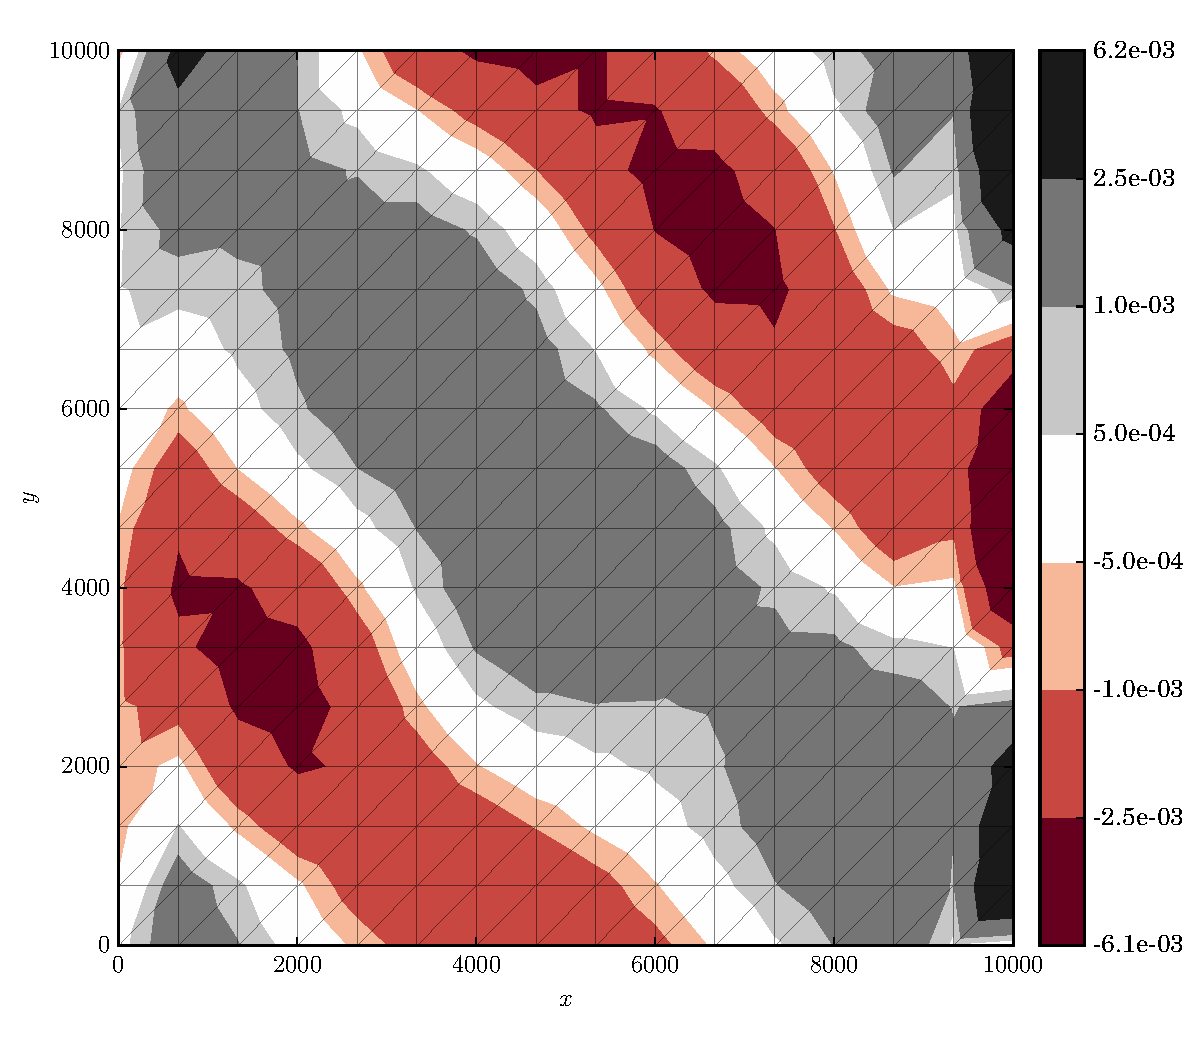
\includegraphics[width=0.3\linewidth]{images/momentum/ISMIP_HOM_A/medium/BP/divU.pdf}
                                                    
    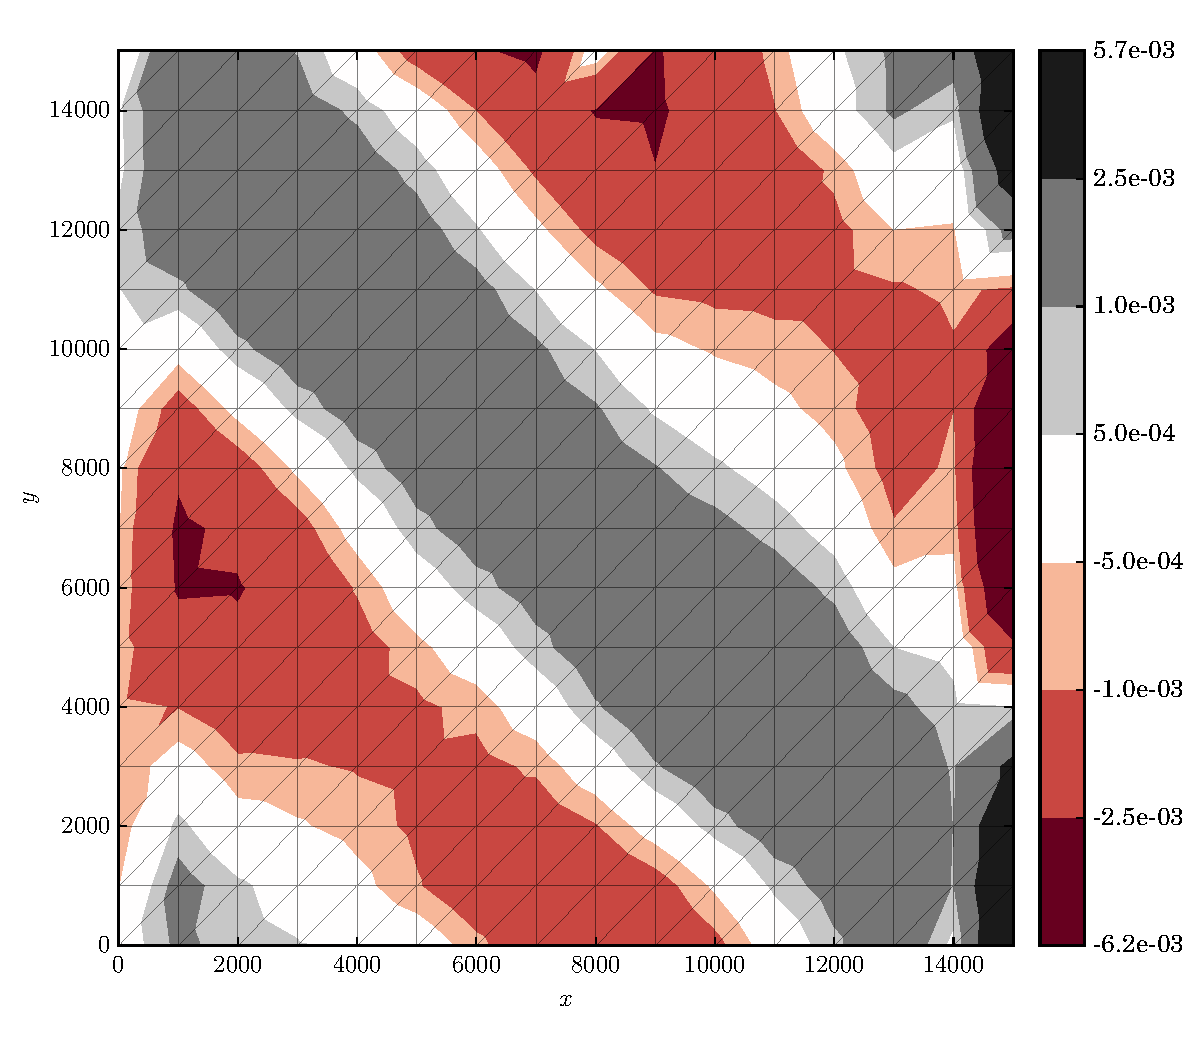
\includegraphics[width=0.3\linewidth]{images/momentum/ISMIP_HOM_A/large/FS/divU.pdf}
    \quad                                           
    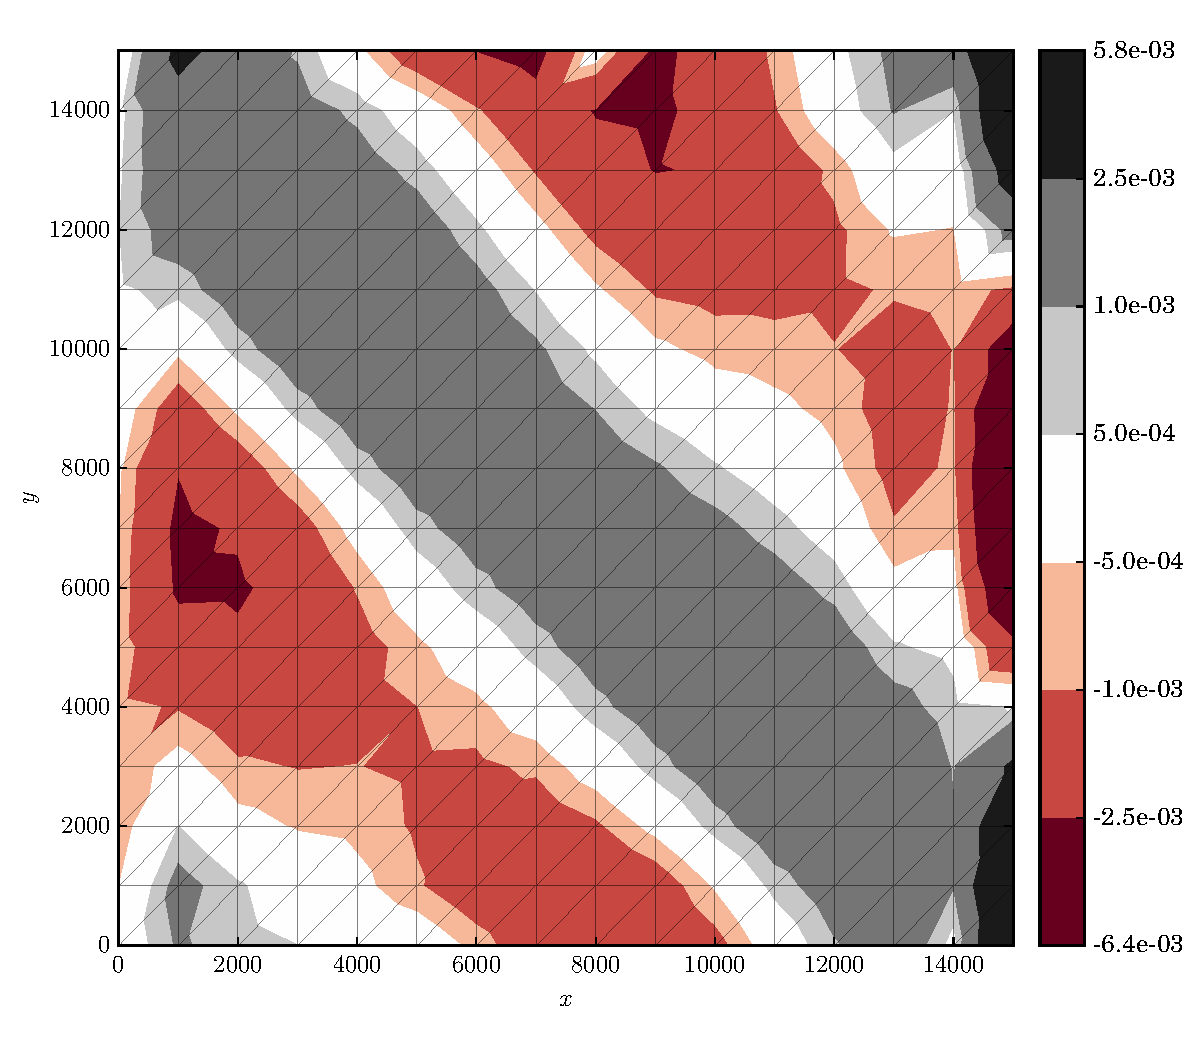
\includegraphics[width=0.3\linewidth]{images/momentum/ISMIP_HOM_A/large/RS/divU.pdf}
    \quad                                           
    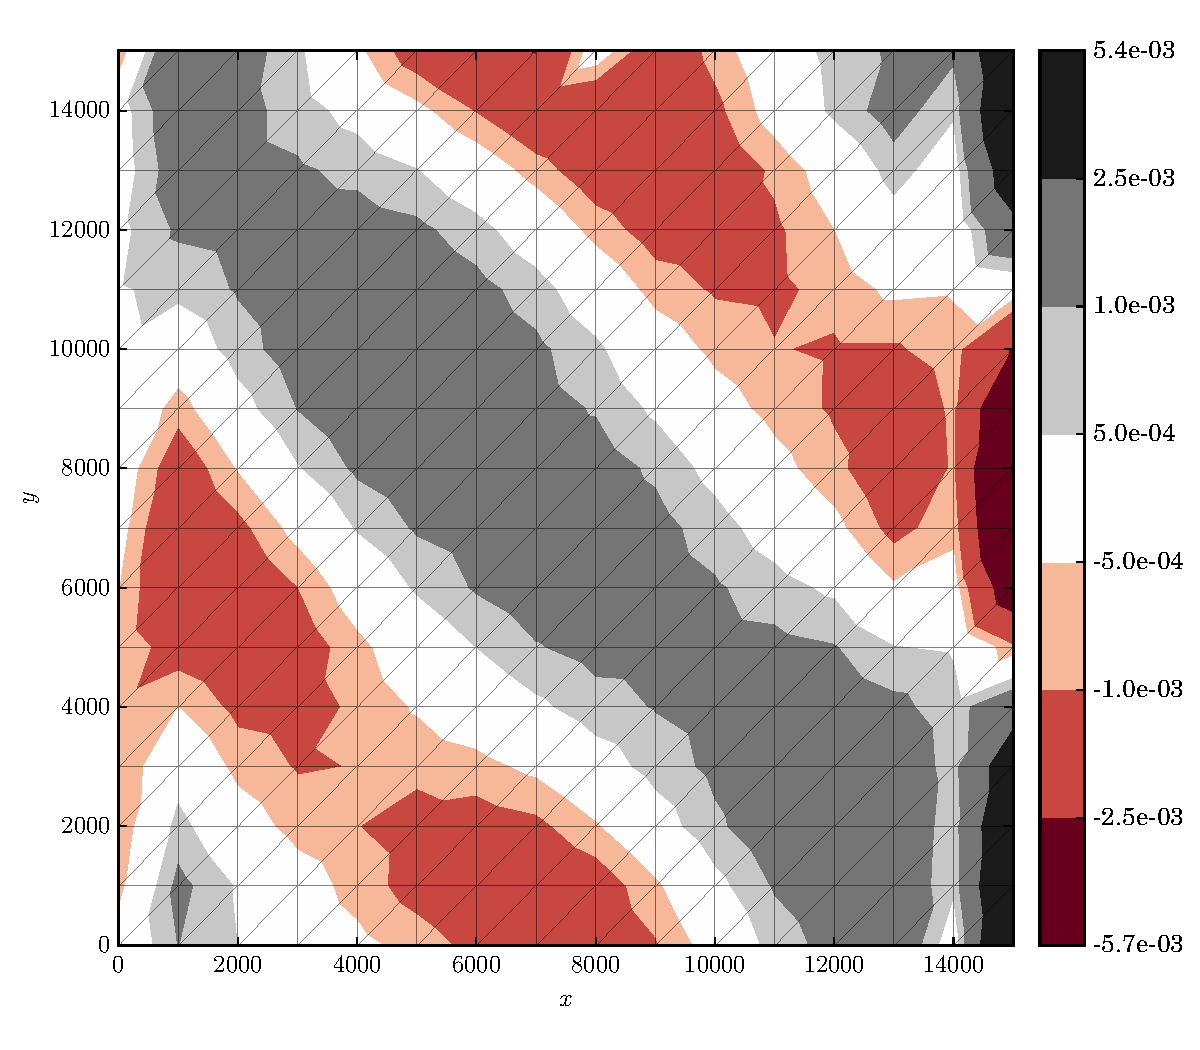
\includegraphics[width=0.3\linewidth]{images/momentum/ISMIP_HOM_A/large/BP/divU.pdf}

  \caption[ISMIP-HOM momentum experiment velocity divergence]{Basal velocity divergence $\nabla \cdot \rankone{u} |_B$ for the ISMIP-HOM test experiment using a $5 \times 5$ square km grid (first row), $8 \times 8$ km$^2$ grid (second row), $10 \times 10$ km$^2$ grid (third row), and $15 \times 15$ km$^2$ grid (fourth row).  The left column are results obtained using the full-Stokes model from \S \ref{ssn_full_stokes}, the middle column using the reformulated-Stokes model of \S \ref{ssn_reformulated_stokes}, and the right column was generated using the first-order model from \S \ref{ssn_first_order}. The color scale across each column is made identical for ease of comparison.}
  \label{ismip_hom_a_divergence}
\end{figure*}

\begin{figure*}
  \centering

    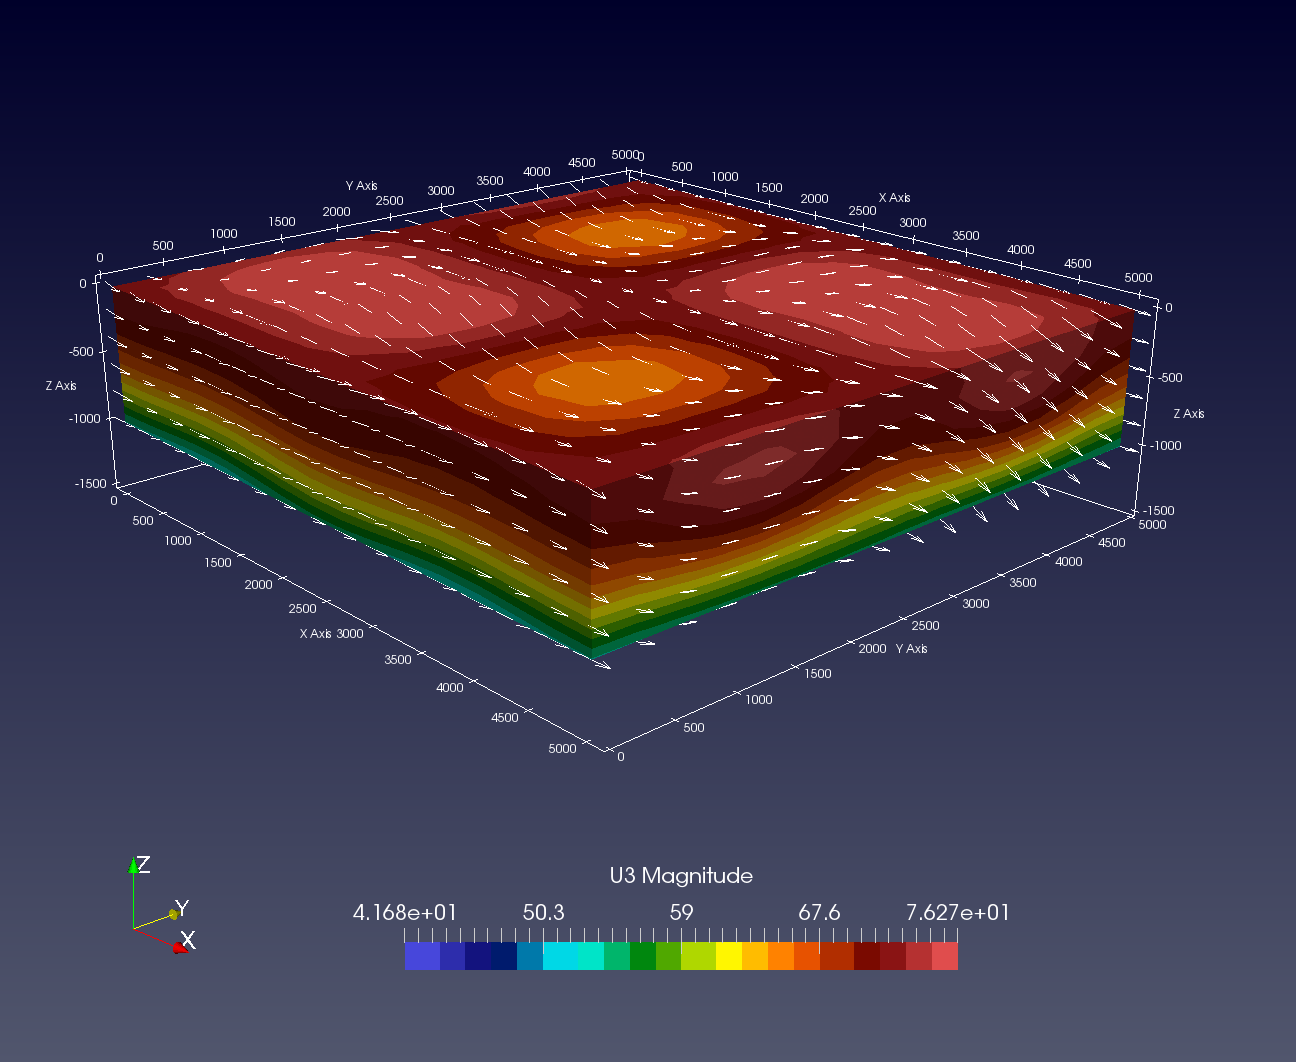
\includegraphics[width=0.7\linewidth]{images/momentum/ISMIP_HOM_A/paraview/FS_top.png}

    \vspace{10mm}

    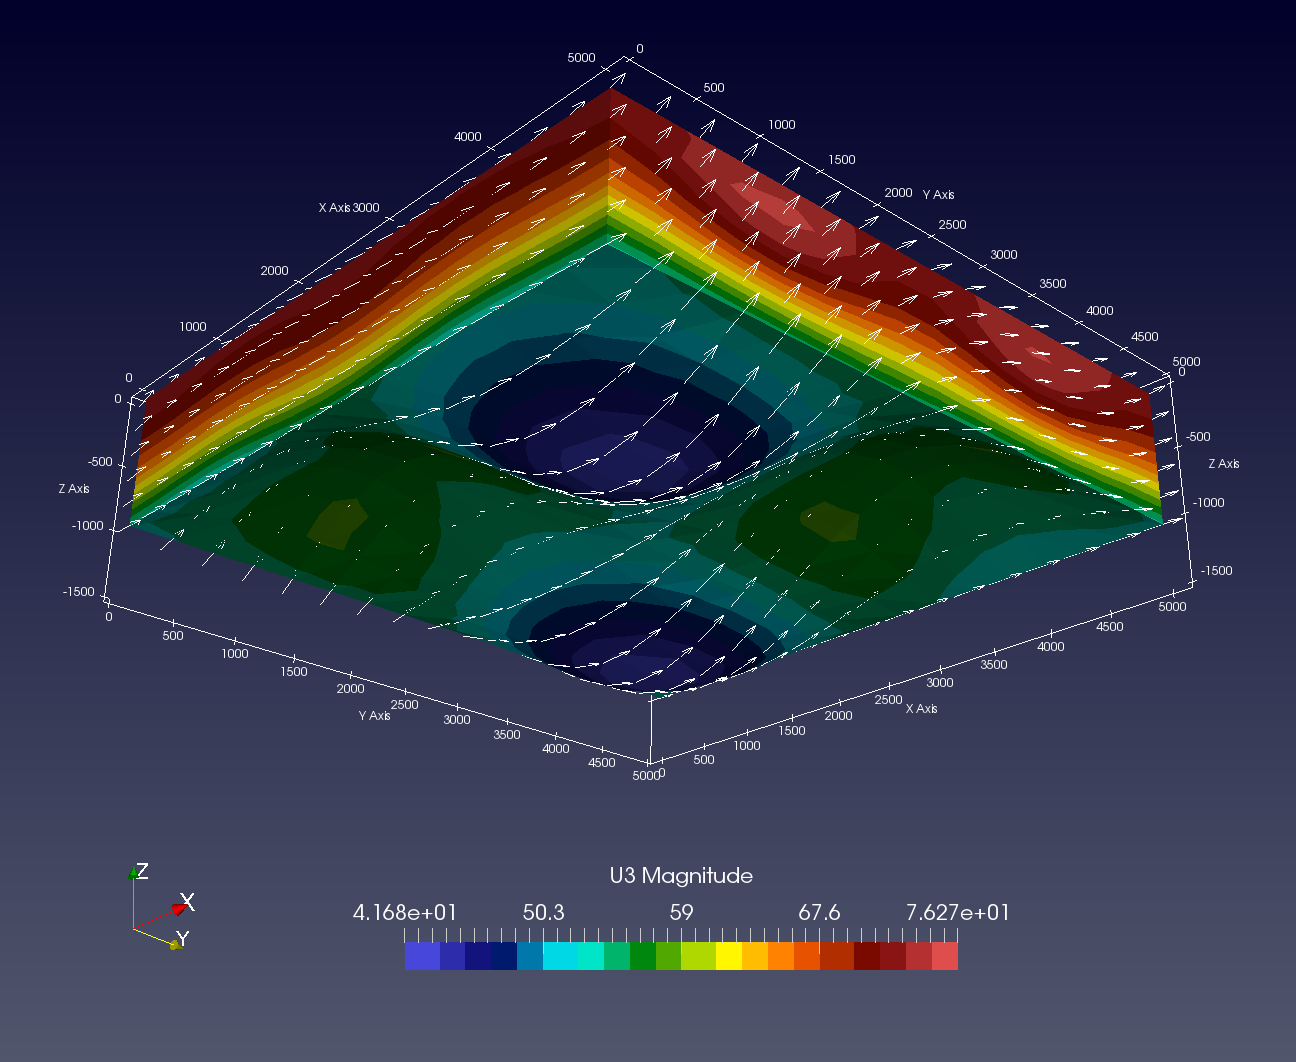
\includegraphics[width=0.7\linewidth]{images/momentum/ISMIP_HOM_A/paraview/FS_bottom.png}

    \caption[Three-dimensional ISMIP-HOM momentum solution]{Full-Stokes velocity $\rankone{u}$ view from above (top) and below (bottom) with a domain of $5 \times 5$ square km.}

  \label{ismip_hom_a_paraview}
\end{figure*}

\begin{figure*}
  \centering

    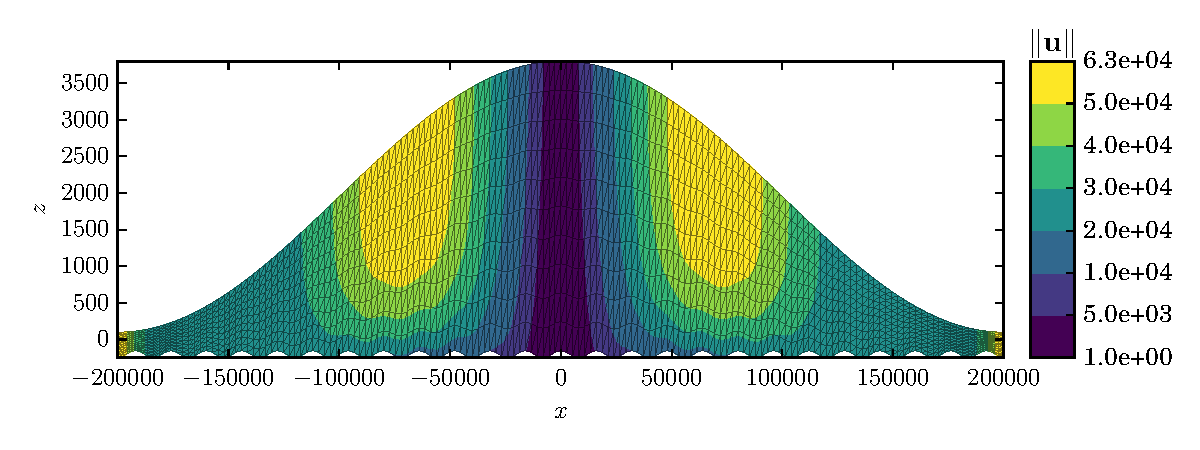
\includegraphics[width=\linewidth]{images/momentum/plane_strain/U_mag.pdf}
    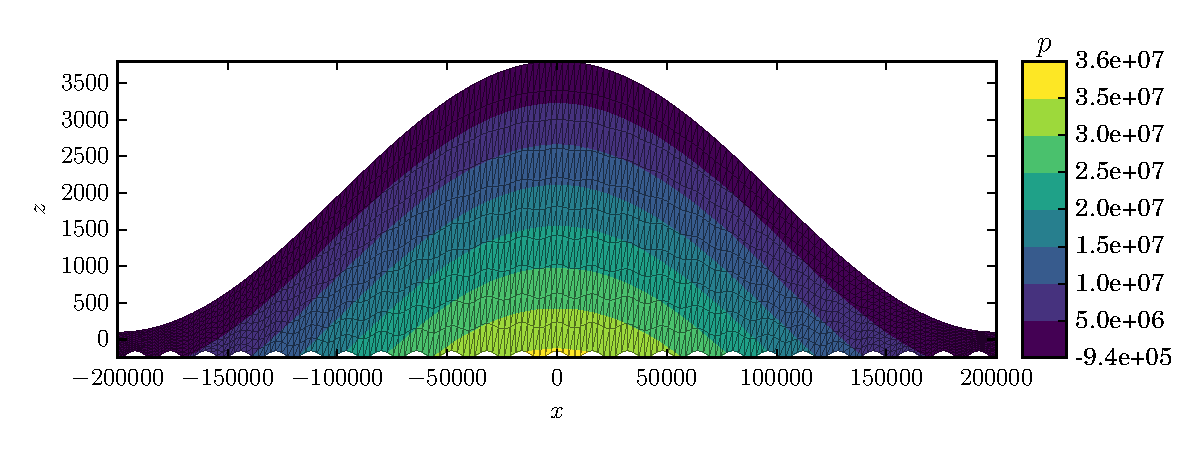
\includegraphics[width=\linewidth]{images/momentum/plane_strain/p.pdf}
    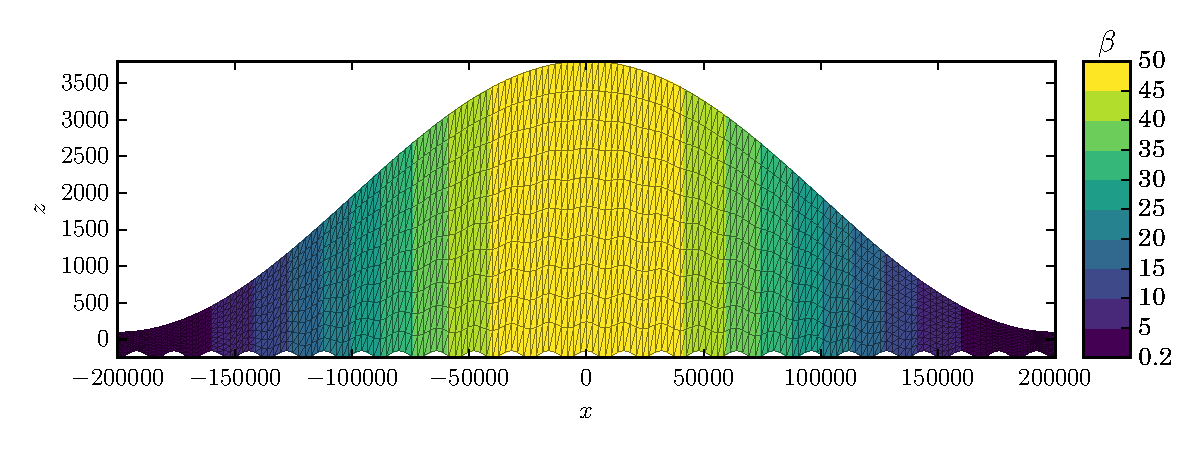
\includegraphics[width=\linewidth]{images/momentum/plane_strain/beta.pdf}

  \caption[Plane-strain momentum experiment solution]{The plane-strain profile results for the simulation outlined by \S \ref{ssn_plane_strain_simulation}; velocity magnitude $\Vert \rankone{u} \Vert$ (top), pressure $p$ (middle), and prescribed basal traction $\beta$ (bottom).}
  \label{plane_strain_image}
\end{figure*}
